\documentclass[12pt,a4paper]{report}

% Compilat cu LuaLaTeX: text Unicode nativ => diacriticele se copiază corect din PDF.
\usepackage{fontspec} % fonturi OpenType Unicode
\setmainfont{Latin Modern Roman}
\setsansfont{Latin Modern Sans}
\setmonofont{Latin Modern Mono}
\usepackage[romanian]{babel} % setări pentru limba română
\renewcommand\familydefault{\sfdefault} % sans serif

\usepackage[margin=2.54cm]{geometry}	% dimensiuni pagină și margini
\usepackage{graphicx} % support the \includegraphics command and options
\usepackage{float} % specificatorul [H] pentru plasare fixă a figurilor/tabelelor
\usepackage{needspace} % păstrează blocuri (listinguri) împreună la capăt de pagină

% formatting sections and subsections
\usepackage{textcase}
\usepackage[titletoc, title]{appendix}
\usepackage{titlesec}
\titleformat{\chapter}{\large\bfseries\MakeUppercase}{\thechapter}{2ex}{}[\vspace*{-1cm}]
\titleformat*{\section}{\large\bfseries}
\titleformat*{\subsection}{\large\bfseries}
\titleformat*{\subsubsection}{\large\bfseries}

\usepackage{chngcntr}
\counterwithout{figure}{chapter} % no chapter number in figure labels
\counterwithout{table}{chapter} % no chapter number in table labels
\counterwithout{equation}{chapter} % no chapter number in equation labels

\usepackage{booktabs} % for much better looking tables
\usepackage{url} % Useful for inserting web links nicely
\usepackage[bookmarks,unicode,hidelinks]{hyperref}

\usepackage{array} % for better arrays (eg matrices) in maths
\usepackage{paralist} % very flexible & customisable lists (eg. enumerate/itemize, etc.)
\usepackage{verbatim} % adds environment for commenting out blocks of text & for better verbatim
\usepackage{subfig} % make it possible to include more than one captioned figure/table in a single float
\captionsetup{justification=centering,belowskip=12pt,aboveskip=8pt} % legende centrate + spațiu sub legendă
\usepackage{enumitem}

% --- Plasarea floturilor: împachetează mai dens, evită pagini cu un singur flot ---
\renewcommand{\topfraction}{0.9}
\renewcommand{\bottomfraction}{0.85}
\renewcommand{\textfraction}{0.07}
\renewcommand{\floatpagefraction}{0.7}
\setcounter{topnumber}{3}
\setcounter{bottomnumber}{2}
\setcounter{totalnumber}{5}
% --- Evită rânduri văduve/orfane la capăt de pagină ---
\widowpenalty=10000
\clubpenalty=10000

% --- Listinguri de cod -------------------------------------------------
\usepackage{xcolor}
\usepackage{listings}
\definecolor{codebg}{gray}{0.97}
\definecolor{codekw}{RGB}{63,94,132}
\definecolor{codecomment}{RGB}{99,140,60}
\definecolor{codestr}{RGB}{170,90,40}
\definecolor{coderule}{gray}{0.75}
\lstdefinestyle{appmesh}{
  basicstyle=\footnotesize\ttfamily,
  backgroundcolor=\color{codebg},
  keywordstyle=\color{codekw},
  commentstyle=\color{codecomment}\itshape,
  stringstyle=\color{codestr},
  numbers=none,
  frame=single, framesep=4pt, rulecolor=\color{coderule},
  breaklines=true, breakatwhitespace=true,
  showstringspaces=false, tabsize=2,
  aboveskip=1.2em, belowskip=0.4em,
  columns=fullflexible, keepspaces=true,
}
\lstset{style=appmesh}

% --- Placeholder pentru screenshot-uri (de inlocuit cu \includegraphics) ---
\newcommand{\screenshotph}[2]{%
  \setlength{\fboxsep}{0pt}%
  \fcolorbox{coderule}{codebg}{\parbox[c][#1][c]{0.88\textwidth}{%
    \centering\color{gray}\itshape[ screenshot de adăugat ]\\[0.5em]\normalfont\small\color{gray} #2}}%
}
\setlist{noitemsep}

%%% HEADERS & FOOTERS
\usepackage{fancyhdr}
\pagestyle{empty}
\renewcommand{\headrulewidth}{0pt}
\renewcommand{\footrulewidth}{0pt}
\lhead{}\chead{}\rhead{}
\lfoot{}\cfoot{\thepage}\rfoot{}

\newcommand{\HeaderLineSpace}{-0.25cm}
\newcommand{\UniTextRO}{UNIVERSITATEA NAȚIONALĂ DE ȘTIINȚĂ ȘI TEHNOLOGIE \\[\HeaderLineSpace]
POLITEHNICA BUCUREȘTI \\[0.22cm]
FACULTATEA DE AUTOMATICĂ ȘI CALCULATOARE \\[\HeaderLineSpace]
DEPARTAMENTUL DE CALCULATOARE\\}
\newcommand{\DiplomaRO}{LUCRARE DE DISERTAȚIE}
\newcommand{\AdvisorRO}{Coordonator științific:}
\newcommand{\BucRO}{BUCUREȘTI}

\newcommand{\UniTextEN}{NATIONAL UNIVERSITY OF SCIENCE AND TECHNOLOGY \\[\HeaderLineSpace]
POLITEHNICA BUCHAREST \\[0.22cm]
FACULTY OF AUTOMATIC CONTROL AND COMPUTERS \\[\HeaderLineSpace]
COMPUTER SCIENCE AND ENGINEERING DEPARTMENT\\}
\newcommand{\DiplomaEN}{MASTER'S THESIS}
\newcommand{\AdvisorEN}{Thesis advisor:}
\newcommand{\BucEN}{BUCHAREST}

\newcommand{\frontPage}[6]{
\begin{titlepage}
\begin{center}
{\Large #1}  % header (university, faculty, department)
\vspace{50pt}
\begin{tabular}{p{6cm}p{4cm}}

\includegraphics[scale=0.8]{pics/upb-logo.jpg} &
	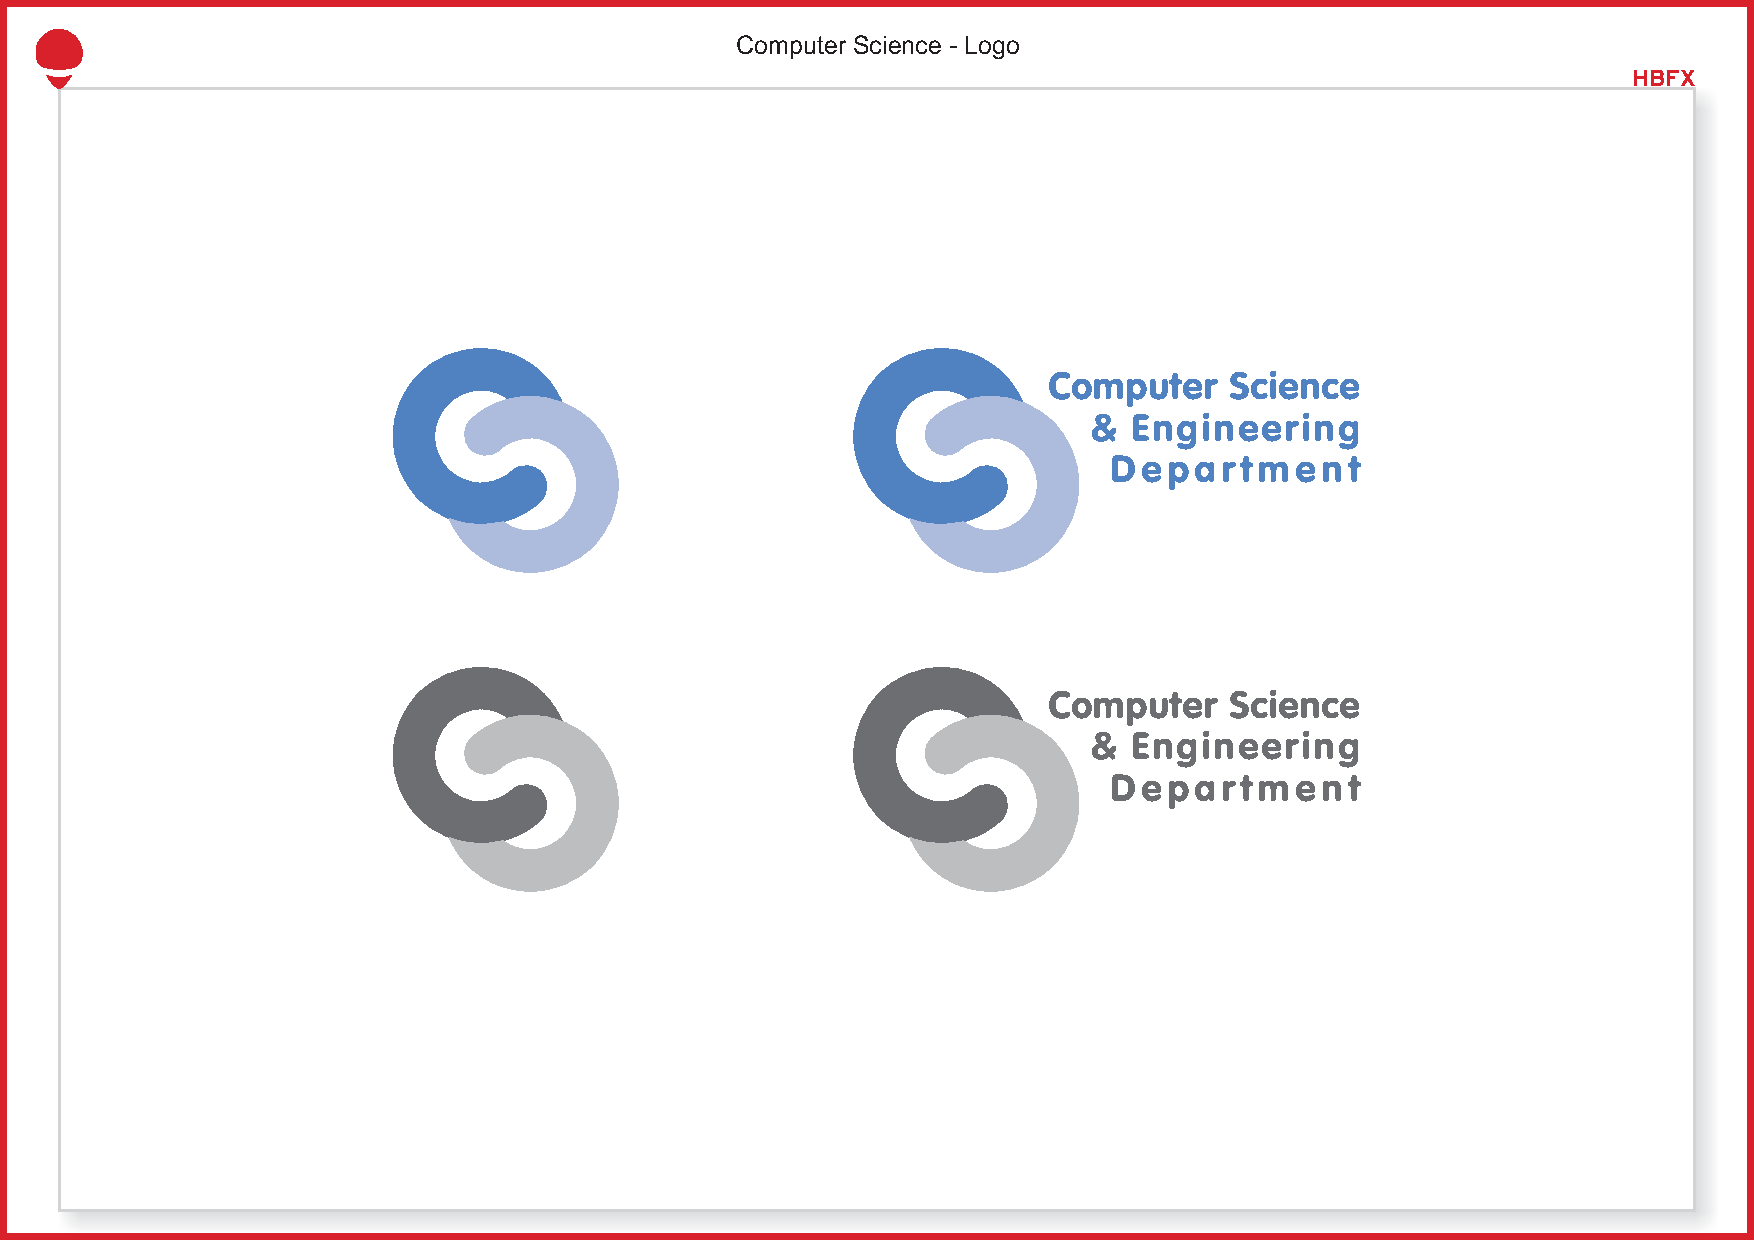
\includegraphics[scale=0.5,trim={14cm 11cm 2cm 5cm},clip=true]{pics/cs-logo.pdf}
\end{tabular}

\vspace{105pt}
{\Huge #2}\\                           % diploma project text
\vspace{40pt}
{\Large #3}\\ \vspace{0pt}  % project title
{\Large #4}\\                          % project subtitle
\vspace{40pt}
{\LARGE \Name}\\                   % student name
\end{center}
\vspace{60pt}
\begin{tabular*}{\textwidth}{@{\extracolsep{\fill}}p{6cm}r}
&{\large\textbf{#5}}\vspace{10pt}\\      % scientific advisor
&{\large \Advisor}                                    % advisor name
\end{tabular*}
\vspace{20pt}
\begin{center}
{\large\textbf{#6}}\\                                % bucharest
\vspace{0pt}
{\normalsize \Year}
\end{center}
\end{titlepage}
}

\newcommand{\frontPageRO}{\frontPage{\UniTextRO}{\DiplomaRO}{\ProjectTitleRO}{\ProjectSubtitleRO}{\AdvisorRO}{\BucRO}}
\newcommand{\frontPageEN}{\frontPage{\UniTextEN}{\DiplomaEN}{\ProjectTitleEN}{\ProjectSubtitleEN}{\AdvisorEN}{\BucEN}}

\linespread{1.15}
\setlength\parindent{0pt}
\setlength\parskip{.28cm}

%% Abstract macro
\newcommand{\AbstractPage}{
\begin{titlepage}
\textbf{\large SINOPSIS}\par
\AbstractRO\par\vfill
\textbf{\large ABSTRACT}\par
\AbstractEN \vfill
\end{titlepage}
}

%% Thank you macro
\newcommand{\ThanksPage}{
\begin{titlepage}
{\noindent \large\textbf{MULȚUMIRI}}\\
\Thanks
\end{titlepage}
}

%%
%%   Câmpurile de mai jos trebuie modificate de autor.
%%
\newcommand{\ProjectTitleRO}{Platformă de gestionare a aplicațiilor web guvernamentale}
\newcommand{\ProjectSubtitleRO}{~}
\newcommand{\ProjectTitleEN}{Platform for Managing Governmental Web Applications}
\newcommand{\ProjectSubtitleEN}{~}
\newcommand{\Name}{Chiru Cristian-Valentin}
\newcommand{\Advisor}{Prof. Dr. Ing. Nirvana Popescu}
\newcommand{\Year}{2026}

% Setări document
\title{Lucrare de disertație}
\author{\Name}
\date{\Year}

%%
%%   Câmpurile aferente rezumatului
%%
\newcommand{\AbstractRO}{Administrația publică oferă astăzi un număr tot mai mare de servicii prin intermediul aplicațiilor web, de la portaluri informative până la servicii de urgență. Aceste aplicații trebuie să fie disponibile permanent, să reziste la creșteri bruște de trafic și la căderi de infrastructură, însă provizionarea și operarea lor presupun un efort tehnic repetitiv și predispus la erori. Lucrarea de față prezintă AppMesh, o platformă self-service care automatizează integral punerea în funcțiune a aplicațiilor web guvernamentale în cloud și gestionează traficul către acestea. Platforma combină o consolă web de administrare, un load balancer multi-region custom, cu rutare pe baza path-ului și failover automat în caz de defect, precum și o direcționare globală a utilizatorilor către cea mai apropiată regiune. Soluția a fost implementată și validată pe o infrastructură reală, găzduind servicii guvernamentale demonstrative pentru ambulanță și poliție.}

\newcommand{\AbstractEN}{Public administration delivers an increasing number of services through web applications, ranging from informational portals to emergency services. These applications must be permanently available and must withstand sudden traffic spikes and infrastructure failures, yet provisioning and operating them involves repetitive, error-prone technical work. This thesis presents AppMesh, a self-service platform that fully automates the deployment of governmental web applications in the cloud and subsequently manages the traffic directed to them. The platform combines a web administration console, a custom multi-region load balancer with path-based routing and automatic failover, and global steering of users towards the nearest region. The solution was implemented and validated on real infrastructure, hosting demonstrative governmental services for ambulance and police.}

%%
%%   Câmpul aferent paginii de mulțumiri
%%
\newcommand{\Thanks}{Doresc să îi mulțumesc doamnei Prof. Dr. Ing. Nirvana Popescu pentru îndrumarea și sprijinul acordate pe parcursul realizării acestei lucrări.}

\begin{document}

\frontPageRO
\frontPageEN

\begingroup
\linespread{1}
\tableofcontents
\endgroup

\AbstractPage

\ThanksPage

% ====================================================================
%  CAPITOLUL 1 — INTRODUCERE
% ====================================================================
\chapter{Introducere}\pagestyle{fancy}

Digitalizarea serviciilor publice a transformat modul în care cetățenii interacționează cu administrația: tot mai multe activități, de la obținerea unor documente până la solicitarea ajutorului în situații de urgență, sunt mediate de aplicații web. Acest capitol introduce contextul în care se înscrie lucrarea, problema pe care o adresează, obiectivele propuse, o privire de ansamblu asupra soluției și a rezultatelor obținute, încheindu-se cu descrierea structurii documentului.

\section{Context}
Instituțiile administrației publice furnizează în prezent o gamă largă de servicii prin intermediul aplicațiilor web, susținute în mod obișnuit de infrastructură găzduită în cloud~\cite{nist-cloud}. Spre deosebire de o aplicație comercială obișnuită, un serviciu public are particularitatea că adresabilitatea sa este universală (orice cetățean poate fi, la un moment dat, utilizatorul lui), iar întreruperea funcționării poate avea consecințe directe asupra siguranței și a încrederii publice. Cazul serviciilor de urgență este edificator: un portal prin care se solicită intervenția unei ambulanțe sau a poliției trebuie să rămână accesibil indiferent de ora din zi, de volumul de cereri sau de eventuale defecțiuni ale infrastructurii subiacente.

Pentru a satisface aceste cerințe, aplicațiile moderne sunt rulate pe mai multe servere și, frecvent, în mai multe regiuni geografice, traficul fiind distribuit între acestea de componente specializate numite \emph{load balancers}~\cite{nginx-lb}. Distribuirea geografică reduce latența percepută de utilizatori, apropiind serviciul de aceștia, și asigură continuitatea funcționării atunci când o întreagă regiune devine indisponibilă. Furnizorii mari de cloud și rețelele de distribuție a conținutului oferă mecanisme de direcționare globală a traficului bazate pe proximitate și pe starea de sănătate a serverelor~\cite{cloudflare-lb}.

\section{Problema}
Deși componentele necesare pentru a rula o aplicație web disponibilă și scalabilă există și sunt mature, asamblarea lor pentru fiecare aplicație în parte rămâne o sarcină laborioasă. Punerea în funcțiune a unui singur serviciu presupune, în practică, configurarea coordonată a numeroase resurse: rețele și reguli de securitate, roluri de acces, șabloane pentru mașini virtuale, grupuri de scalare automată, load balancere la nivel de regiune, înregistrări DNS și health-check-uri. Aceste operațiuni sunt repetitive, dependente între ele și predispuse la erori atunci când sunt efectuate manual.

Problema se amplifică atunci când o instituție trebuie să administreze nu una, ci un portofoliu întreg de aplicații, fiecare cu propriul ciclu de viață și cu necesitatea de a fi prezentă în mai multe regiuni. În absența unei abordări unitare, fiecare punere în funcțiune devine un proces izolat, dificil de reprodus și de monitorizat, iar reacția la o defecțiune depinde de intervenția manuală a unui operator. Lipsa unui punct central de control face dificilă atât observarea stării reale a sistemului, cât și aplicarea consecventă a deciziilor de rutare a traficului.

\section{Obiective}
Obiectivul principal al lucrării este proiectarea și implementarea unei platforme care să unifice, sub o singură interfață, întregul ciclu de viață al aplicațiilor web guvernamentale, de la punerea în funcțiune până la administrarea traficului în exploatare. Pentru atingerea acestui obiectiv general au fost urmărite următoarele obiective specifice:

\begin{itemize}
	\item automatizarea integrală a punerii în funcțiune a unei aplicații web în cloud, pornind de la o singură acțiune efectuată din interfața de administrare, fără configurare manuală a resurselor de infrastructură;
	\item realizarea unui load balancer multi-region custom, capabil să direcționeze cererile pe baza path-ului și să facă failover automat al traficului către o regiune alternativă atunci când regiunea preferată devine indisponibilă;
	\item direcționarea globală a utilizatorilor către regiunea cea mai apropiată, cu reorientarea automată a acestora în cazul în care regiunea respectivă nu mai răspunde;
	\item menținerea unei surse unice și consecvente de adevăr privind configurația și starea aplicațiilor administrate, accesibilă printr-o consolă centralizată;
	\item validarea soluției pe o infrastructură reală, prin găzduirea unor servicii guvernamentale reprezentative.
\end{itemize}

\section{Soluția propusă}
Soluția propusă, denumită AppMesh, este o platformă care separă clar planul de control de planul de date. Planul de control este reprezentat de o consolă web de administrare prin care un operator definește aplicațiile dorite și regiunile în care acestea trebuie să ruleze. Pe baza acestor decizii, consola provizionează automat toate resursele necesare în cloud și menține o evidență centralizată a configurației și a stării fiecărei aplicații.

Planul de date este format dintr-un load balancer custom, deploiat în fiecare regiune, care primește cererile utilizatorilor și le direcționează către instanțele aplicației corespunzătoare. Acesta selectează cererile în funcție de path-ul solicitat, preferă regiunea în care se află și face failover al traficului către o altă regiune atunci când detectează defecțiuni, evitând regiunile cu probleme până la remedierea problemelor din acestea. La nivel global, utilizatorii sunt orientați către cel mai apropiat punct de intrare, ceea ce reduce latența și permite redirecționarea automată în caz de indisponibilitate. Întreaga configurație a load balancerelor este derivată din evidența centralizată menținută de consolă, astfel încât planul de date reflectă în permanență deciziile luate în planul de control.

\section{Rezultatele obținute}
Platforma a fost implementată complet și pusă în funcțiune pe o infrastructură reală, folosind serviciile Amazon Web Services (AWS) împreună cu rețeaua globală Cloudflare pentru direcționarea traficului. Prin intermediul consolei, o aplicație web poate fi pusă în funcțiune integral automat, fără ca operatorul să configureze manual vreo resursă de infrastructură. Load balancer-ul custom rutează corect cererile către serviciile administrate și face failover către o regiune alternativă atunci când regiunea preferată devine indisponibilă, fără ca utilizatorul final să fie afectat.

Funcționalitatea platformei a fost demonstrată prin găzduirea unor servicii guvernamentale reprezentative (un serviciu de ambulanță și unul de poliție), fiecare expunând regiunea și instanța care îl deservesc, ceea ce face vizibilă în mod direct comportarea mecanismului de distribuție și de failover. Rezultatele confirmă că o instituție poate administra un portofoliu de aplicații web disponibile și scalabile dintr-un singur punct de control, cu un efort operațional considerabil redus față de gestionarea manuală a fiecărei componente.

\section{Structura lucrării}
Lucrarea este organizată în opt capitole. Capitolul de față introduce contextul, problema, obiectivele și soluția propusă. Capitolul al doilea analizează și specifică cerințele platformei, formulând lista de funcționalități care rezultă din acestea. Capitolul al treilea prezintă abordările existente pentru distribuirea traficului și administrarea aplicațiilor în cloud, poziționând soluția propusă față de acestea și descriind tehnologiile utilizate. Capitolul al patrulea detaliază soluția propusă, prin arhitectura sa de ansamblu și deciziile de proiectare. Capitolul al cincilea tratează aspectele de implementare, insistând asupra elementelor care au prezentat dificultăți tehnice deosebite. Capitolul al șaselea descrie testarea și validarea platformei, prin suita automată de testare în patru faze și prin verificarea independentă a efectelor asupra infrastructurii. Capitolul al șaptelea prezintă evaluarea experimentală, cu metrici cantitative măsurate pe platforma în funcțiune. Capitolul al optulea prezintă concluziile și direcțiile de dezvoltare ulterioară.

% ====================================================================
%  CAPITOLUL 2.ANALIZA SI SPECIFICAREA CERINTELOR
% ====================================================================
\chapter{Analiza și specificarea cerințelor}

Acest capitol stabilește ce trebuie să realizeze platforma, pornind de la actorii care interacționează cu ea și de la scenariile concrete de utilizare. Din analiza acestora sunt derivate cerințele funcționale și nefuncționale, capitolul încheindu-se cu lista de funcționalități care rezultă din ele și care va ghida proiectarea soluției.

\section{Actori și scenarii de utilizare}
Platforma deservește două categorii de actori cu nevoi distincte. \textbf{Operatorul} este administratorul tehnic al unei instituții, care folosește consola pentru a pune în funcțiune și a administra aplicațiile din portofoliu, regiunile active și conturile de acces. \textbf{Utilizatorul final} este cetățeanul care accesează un serviciu găzduit și care se așteaptă ca acesta să fie disponibil permanent și să răspundă rapid, fără a fi conștient de infrastructura din spate.

Din interacțiunea acestor actori cu sistemul rezultă următoarele scenarii reprezentative:

\begin{itemize}
	\item \textbf{S1. Punerea în funcțiune a unei aplicații.} Operatorul încarcă artefactul unei aplicații și declară regiunea în care trebuie să ruleze. Platforma provizionează automat toate resursele necesare și raportează progresul pas cu pas, până când aplicația devine accesibilă.
	\item \textbf{S2. Extinderea unei aplicații în mai multe regiuni.} Pentru un serviciu deja funcțional, operatorul adaugă o regiune suplimentară, iar platforma replică automat aplicația acolo și actualizează configurația de rutare.
	\item \textbf{S3. Defectarea unei regiuni.} Atunci când regiunea preferată a unui serviciu devine indisponibilă, traficul trebuie să fie redirecționat automat, prin failover, către o regiune funcțională, fără intervenția operatorului și fără impact vizibil pentru utilizatorul final.
	\item \textbf{S4. Variația sarcinii.} La creșterea volumului de cereri, numărul de instanțe ale unei aplicații trebuie să crească automat, iar la scăderea acestuia să revină, pentru a echilibra disponibilitatea și costul.
	\item \textbf{S5. Retragerea unei aplicații sau a unei regiuni.} Operatorul poate elimina o regiune a unui serviciu sau serviciul în întregime, platforma eliberând automat toate resursele asociate.
	\item \textbf{S6. Administrarea accesului.} Operatorul administrator gestionează conturile celorlalți operatori care pot folosi consola.
\end{itemize}

Figura~\ref{fig:usecase} sintetizează aceste scenarii sub forma unei diagrame use-case, evidențiind cazurile de utilizare inițiate de operator și pe cele care țin de accesul utilizatorului final, împreună cu comportamentele automate de failover și de scalare pe care platforma le declanșează în cursul deservirii traficului.

\begin{figure}[H]
\centering
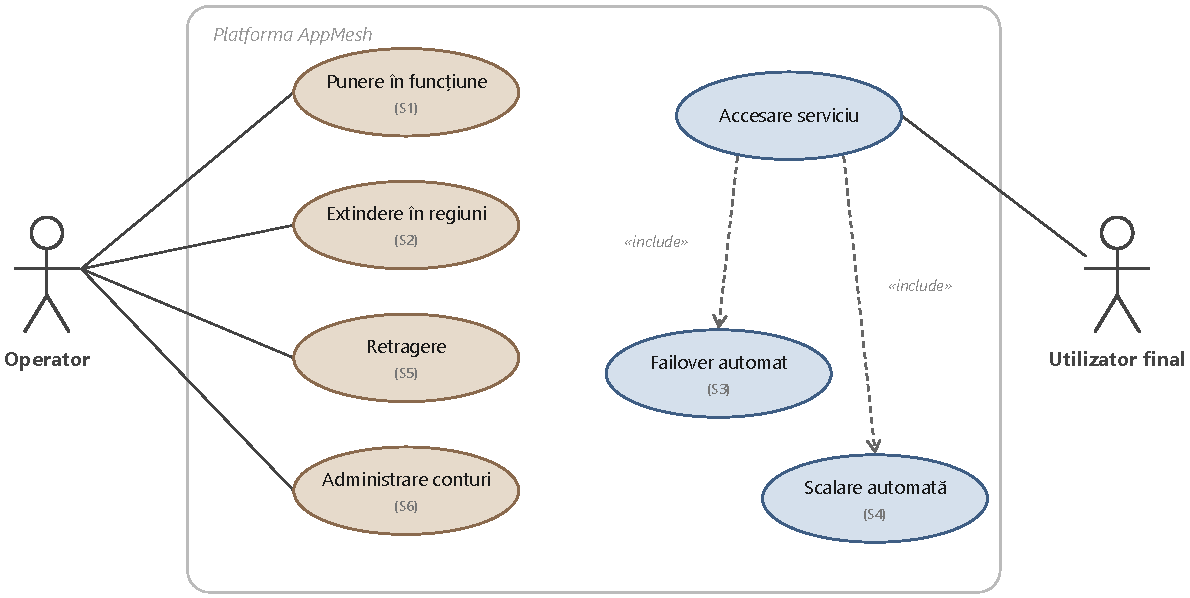
\includegraphics[width=0.9\textwidth]{pics/fig_usecase.pdf}
\caption{Diagrama use-case a platformei: cazurile de utilizare ale operatorului și ale utilizatorului final}
\label{fig:usecase}
\end{figure}

\section{Cerințe funcționale}
Pe baza scenariilor de mai sus au fost specificate următoarele cerințe funcționale:

\begin{itemize}
	\item \textbf{CF1.} Sistemul trebuie să pună în funcțiune o aplicație web pornind de la o singură acțiune din consolă, provizionând automat întregul lanț de resurse (rețea și reguli de securitate, rol de acces, launch template, Auto Scaling Group, target group, regulă de rutare pe load balancer-ul regional, înregistrare DNS) fără configurare manuală.
	\item \textbf{CF2.} Sistemul trebuie să afișeze progresul fiecărei etape din punerea în funcțiune și starea curentă a fiecărei aplicații administrate.
	\item \textbf{CF3.} Sistemul trebuie să permită rularea aceleiași aplicații în mai multe regiuni și gestionarea individuală a fiecărei regiuni.
	\item \textbf{CF4.} Load balancer-ul trebuie să direcționeze cererile către serviciul corect pe baza path-ului din cerere.
	\item \textbf{CF5.} Load balancer-ul trebuie să facă failover automat al traficului către o regiune alternativă atunci când regiunea preferată răspunde cu erori sau nu răspunde, și să evite regiunile defecte până la revenirea lor.
	\item \textbf{CF6.} Sistemul trebuie să direcționeze utilizatorii, la nivel global, către regiunea cea mai apropiată și să îi reorienteze automat atunci când aceasta devine indisponibilă.
	\item \textbf{CF7.} Sistemul trebuie să verifice periodic starea de sănătate a serviciilor prin intermediul health-check-urilor și să folosească rezultatul în deciziile de rutare.
	\item \textbf{CF8.} Sistemul trebuie să mențină o sursă unică și consecventă de adevăr privind configurația și starea aplicațiilor, din care să derive automat configurația load balancer-elor.
	\item \textbf{CF9.} Sistemul trebuie să permită retragerea controlată a unei regiuni sau a unei aplicații, cu eliberarea tuturor resurselor asociate.
	\item \textbf{CF10.} Sistemul trebuie să ofere autentificare și administrarea conturilor de operatori.
\end{itemize}

\section{Cerințe nefuncționale}
Dincolo de funcționalitate, platforma trebuie să satisfacă o serie de cerințe de calitate:

\begin{itemize}
	\item \textbf{Disponibilitate.} Serviciile găzduite trebuie să rămână accesibile chiar și la defectarea unei instanțe sau a unei întregi regiuni, prin redundanță și failover automat.
	\item \textbf{Scalabilitate.} Sistemul trebuie să se adapteze la variații ale sarcinii prin scalare automată orizontală și să permită extinderea în noi regiuni.
	\item \textbf{Performanță.} Direcționarea globală pe baza proximității trebuie să reducă latența percepută, iar overhead-ul introdus de load balancer-ul propriu trebuie să fie redus.
	\item \textbf{Securitate.} Accesul la consolă trebuie protejat prin autentificare, iar credențialele și secretele nu trebuie expuse în artefactele distribuite.
	\item \textbf{Utilizabilitate.} Operatorul trebuie să poată administra întregul portofoliu dintr-o singură interfață, fără cunoștințe aprofundate despre infrastructura subiacentă.
	\item \textbf{Observabilitate.} Starea aplicațiilor, a regiunilor și a deciziilor de rutare trebuie să fie vizibilă operatorului.
	\item \textbf{Cost.} Resursele trebuie dimensionate și eliberate astfel încât să se evite consumul inutil.
\end{itemize}

\section{Lista de funcționalități}
Sintetizând cerințele de mai sus, platforma oferă următoarele funcționalități:

\begin{itemize}
	\item consolă web de administrare cu autentificare și gestionarea conturilor de operatori;
	\item punere în funcțiune complet automatizată a unei aplicații web în cloud, cu raportarea progresului pas cu pas;
	\item extindere și restrângere a unei aplicații pe mai multe regiuni;
	\item load balancer multi-region custom, cu rutare pe baza path-ului și failover automat între regiuni;
	\item direcționare globală a utilizatorilor pe baza proximității, cu reorientare în cazul apariției unor probleme într-o regiune;
	\item monitorizarea sănătății serviciilor prin health-check-uri;
	\item evidență centralizată a configurației și a stării;
	\item scalare automată orizontală a instanțelor fiecărei aplicații;
	\item retragere controlată a regiunilor și a aplicațiilor, cu eliberarea resurselor.
\end{itemize}

% ====================================================================
%  CAPITOLUL 3.ABORDARI EXISTENTE
% ====================================================================
\chapter{Abordări existente}

Problema distribuirii traficului către aplicații web disponibile și scalabile nu este nouă, iar pentru componentele individuale ale acesteia există soluții mature. Acest capitol prezintă principalele categorii de abordări existente, analizează limitările lor în raport cu problema tratată, poziționează soluția propusă față de ele și descrie tehnologiile utilizate în implementare.

\section{Soluții oferite de furnizorii de cloud}
Furnizorii mari de cloud oferă servicii gestionate de distribuție a traficului. La nivel de regiune, serviciile de tip Application Load Balancer rutează cererile către instanțe pe baza host-ului sau a path-ului și efectuează health-check-uri asupra acestora~\cite{aws-elb}. Pentru direcționarea globală există servicii bazate pe DNS, care aleg regiunea în funcție de latență sau de poziția geografică a clientului~\cite{aws-route53}, precum și servicii bazate pe rețeaua anycast a furnizorului, care orientează traficul către cel mai apropiat punct de intrare~\cite{aws-globalaccelerator}.

Aceste servicii sunt robuste și scalabile, însă operează la nivel de infrastructură: ele presupun că aplicația și resursele subiacente au fost deja create și configurate. Combinarea lor pentru a obține o aplicație multi-regiune rămâne o sarcină de orchestrare, realizată de obicei prin descrieri de tip \emph{infrastructure as code}, care trebuie scrise și întreținute separat pentru fiecare aplicație. În plus, ele nu oferă o consolă unitară pentru administrarea unui portofoliu întreg de aplicații și leagă soluția de ecosistemul unui singur furnizor.

\section{Soluții software self-managed}
O a doua categorie o reprezintă load balancer-ele și reverse proxy-urile software, instalate și administrate de utilizator: NGINX~\cite{nginx-lb}, HAProxy~\cite{haproxy} și Envoy~\cite{envoy}. Acestea oferă control fin asupra rutării la nivel de aplicație, health-check-uri și mecanisme de failover, fiind componente foarte performante și larg utilizate.

Limitarea lor în raport cu problema tratată este că reprezintă exclusiv un plan de date: ele direcționează traficul conform unei configurații, dar nu acoperă planul de control. Coordonarea între regiuni, distribuirea consecventă a configurației, automatizarea punerii în funcțiune a aplicațiilor și menținerea unei evidențe centralizate rămân integral în sarcina utilizatorului, care trebuie să le construiască în jurul acestor componente.

\section{Soluții bazate pe DNS}
A treia categorie o constituie soluțiile de tip \emph{global server load balancing} bazate pe DNS, în care direcționarea globală se face prin răspunsul la interogările de rezoluție a numelor: clientul este orientat către cea mai apropiată regiune funcțională în funcție de adresa returnată~\cite{cloudflare-lb}. Acestea sunt eficiente pentru distribuirea geografică a utilizatorilor și sunt folosite de marile platforme online.

Slăbiciunea lor ține de nivelul la care acționează. Deciziile fiind luate la rezoluția DNS, reorientarea la defectarea regiunii depinde de expirarea valorilor de cache de la nivelul clienților și al resolver-elor, ceea ce poate întârzia failover-ul. De asemenea, ele nu oferă rutare pe baza path-ului către servicii distincte și nu administrează ciclul de viață al aplicațiilor din spate.

\section{Poziționarea soluției propuse}
Fiecare categorie de mai sus rezolvă bine o parte din problemă, dar niciuna nu o acoperă integral pentru cazul unui portofoliu de aplicații web guvernamentale administrat de o singură echipă. Soluția propusă combină punctele forte ale acestor abordări într-o platformă unitară: automatizarea punerii în funcțiune specifică platformelor de tip PaaS, un load balancer multi-region custom cu rutare pe path și failover activ specific load balancer-elor software, și direcționarea globală pe baza proximității specifică soluțiilor DNS. Spre deosebire de ele, toate aceste mecanisme sunt conduse dintr-un singur plan de control, cu o sursă centralizată de adevăr din care derivă automat configurația planului de date. Figura~\ref{tab:comparatie} sintetizează această poziționare.

\begin{figure}[H]
\centering
\small\linespread{1.1}
\begin{tabular}{@{}>{\raggedright\arraybackslash}p{5.2cm}
                   *{4}{>{\centering\arraybackslash}p{2.05cm}}@{}}
\toprule
\textbf{Capabilitate} & \textbf{Cloud gestionat} & \textbf{LB software} & \textbf{DNS} & \textbf{Soluția propusă} \\
\midrule
Punere în funcțiune automată        & parțial   & nu        & nu        & \textbf{da} \\
Rutare pe path                      & da        & da        & nu        & \textbf{da} \\
Failover activ între regiuni        & da        & da        & întârziat & \textbf{da} \\
Direcționare globală pe proximitate & da        & nu        & da        & \textbf{da} \\
Plan de control unificat            & nu        & nu        & nu        & \textbf{da} \\
\bottomrule
\end{tabular}
\vspace{4pt}
\caption{Poziționarea soluției propuse față de abordările existente}
\label{tab:comparatie}
\end{figure}

\section{Tehnologii utilizate}
Implementarea platformei se sprijină pe un set de tehnologii alese pentru a se potrivi rolului fiecărei componente.

\textbf{Consola de administrare} este construită în Python cu micro-framework-ul Flask~\cite{flask}, interacțiunea cu serviciile cloud realizându-se prin SDK-ul oficial boto3~\cite{boto3}. Flask a fost preferat unor framework-uri mai ample precum Django datorită amprentei reduse și a libertății în organizarea aplicației, consola fiind în esență un orchestrator în jurul apelurilor către cloud.

\textbf{Load balancer-ul} este implementat folosind Spring Cloud Gateway~\cite{scgateway}, o platformă reactivă, neblocantă, construită pe Spring Boot. Spre deosebire de un load balancer software configurabil precum NGINX sau HAProxy, Spring Cloud Gateway permite definirea de filtre programabile, ceea ce a făcut posibilă implementarea directă, în cod, a logicii de failover între regiuni și a mecanismului de circuit breaker~\cite{nygard-circuitbreaker}, dificil de exprimat printr-o configurație pur declarativă. Configurația de rutare este preluată dinamic din S3 prin SDK-ul AWS pentru Java.

\textbf{Infrastructura} este furnizată de Amazon Web Services: fiecare aplicație rulează pe mașini virtuale EC2 grupate în Auto Scaling Groups, load balancere regionale gestionate (ALB), stocare de obiecte S3 pentru artefacte, configurație și stare, baza de date DynamoDB pentru conturi și metadate, precum și roluri de acces IAM. Direcționarea globală pe baza proximității este realizată cu serviciul de \emph{load balancing} al Cloudflare~\cite{cloudflare-lb}, prin origin pool-uri, health monitors și o politică de rutare bazată pe proximitate.

\textbf{Aplicațiile demonstrative} sunt servicii Spring Boot care expun, pe lângă conținut, regiunea și instanța care le deservesc, făcând vizibil comportamentul mecanismului de distribuție.

% ====================================================================
%  CAPITOLUL 4. SOLUTIA PROPUSA
% ====================================================================
\chapter{Soluția propusă}

Acest capitol descrie arhitectura platformei AppMesh. Sunt prezentate mai întâi structura de ansamblu și principiul de organizare care stă la baza ei, separarea planului de control de planul de date, după care fiecare plan este detaliat: consola de administrare, load balancer-ul multi-region, rutarea traficului și modelul de date care leagă întregul sistem.

\section{Arhitectura de ansamblu}
Din punct de vedere structural, platforma este organizată pe două planuri care funcționează independent în timp. \emph{Planul de control} cuprinde consola de administrație, configurațiile și starea; el este activ atunci când operatorul ia decizii (punerea în funcțiune a unei aplicații, adăugarea unei regiuni, deprovizionarea unui serviciu). \emph{Planul de date} cuprinde componentele care deservesc traficul real al utilizatorilor și funcționează continuu, independent de prezența operatorului. Figura~\ref{fig:arch} prezintă această organizare.

\begin{figure}[H]
\centering
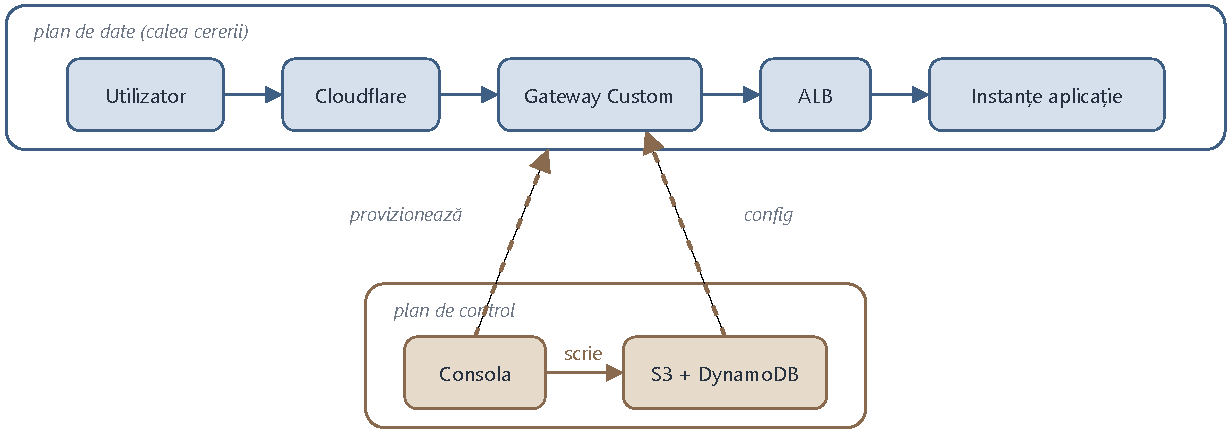
\includegraphics[width=0.92\textwidth]{pics/fig_arhitectura.pdf}
\caption{Arhitectura de ansamblu a platformei: planul de date deservește cererile, planul de control le configurează}
\label{fig:arch}
\end{figure}

Pe calea cererii, un utilizator care accesează platforma este orientat de Cloudflare către gateway-ul din regiunea cea mai apropiată. Gateway-ul reprezintă load balancer-ul custom și alege serviciul corespunzător pe baza path-ului, trimițând cererea, prin ALB (load balancer-ul regional al furnizorului de cloud), către una dintre instanțele aplicației. Această cale este replicată în fiecare regiune adăugată, astfel încât defectarea unei regiuni nu întrerupe serviciul.

Pe latura de control, consola provizionează resursele necesare în cloud și consemnează starea deployment-urilor în DynamoDB. Din această stare, consola derivă configurația de rutare și o publică în S3, sub forma câte unui fișier per regiune, de unde fiecare load balancer își preia periodic propria configurație. Astfel, cele două planuri sunt cuplate slab: ele comunică exclusiv prin configurația din S3, nu prin apeluri directe, ceea ce face ca planul de date să continue să funcționeze chiar dacă planul de control este oprit.

Aceeași arhitectură poate fi privită și pe straturi funcționale suprapuse, de la intrarea în rețea până la planul de control. Figura~\ref{fig:straturi} prezintă această organizare: stratul edge (Cloudflare) direcționează cererea către regiunea cea mai apropiată, stratul de management al traficului (ALB-ul regional și gateway-ul custom) o rutează către serviciul potrivit, iar stratul aplicație o deservește prin instanțele EC2. Sub acestea, stratul de configurație și stare (S3 și DynamoDB) păstrează artefactele, configurația de rutare și starea sistemului, iar stratul de administrare (consola) provizionează resursele și publică configurația.

\begin{figure}[H]
\centering
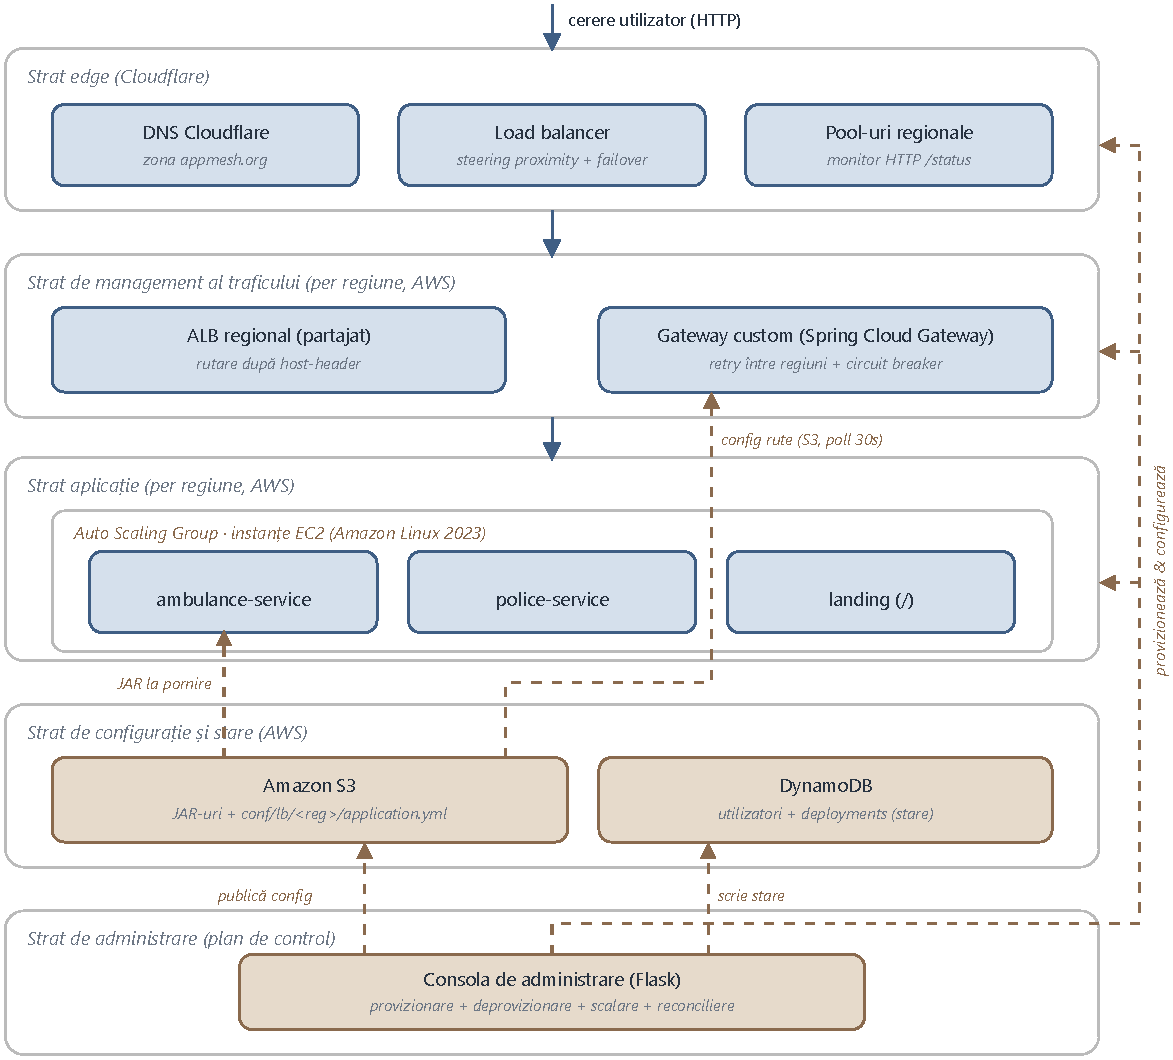
\includegraphics[width=0.74\textwidth]{pics/fig_straturi.pdf}
\caption{Arhitectura platformei pe straturi funcționale}
\label{fig:straturi}
\end{figure}

\section{Separarea planului de control de planul de date}
Planul de control concentrează toată logica de provizionare și de luare a deciziilor, dar nu se află niciodată pe calea critică a unei cereri de la utilizator. Planul de date este simplu și autonom: el citește o configurație declarativă și o aplică, fără a depinde de disponibilitatea consolei.

Avantajul principal al acestei separări este robustețea. O eroare sau o oprire a consolei nu afectează traficul aflat în desfășurare, întrucât gateway-urile dețin deja, local, ultima configurație validă preluată din S3. În plus, comunicarea indirectă prin configurație face ca adăugarea unei noi regiuni să se reducă, din perspectiva planului de date, la apariția unui nou gateway care preia aceeași sursă de configurație, fără modificări de cod sau coordonare explicită între componente.

\section{Planul de control: consola de administrare}
Consola este o aplicație web prin care operatorul administrează întregul portofoliu. Rolul ei nu este acela de a deservi trafic, ci de a implementa deciziile operatorului în resurse concrete de infrastructură și de a oferi o imagine consecventă a stării sistemului.

La punerea în funcțiune a unei aplicații, consola execută, în ordine, un lanț de pași de provizionare: pregătește regulile de securitate și rolul de acces, încarcă artefactul aplicației în S3, creează launch template-ul și Auto Scaling Group-ul, atașează aplicația la load balancer-ul regional printr-o regulă de rutare și creează înregistrarea DNS corespunzătoare, așteptând în final ca aplicația să devină funcțională. Fiecare pas este consemnat, astfel încât operatorul urmărește progresul în timp real, iar în cazul deprovizionării unui serviciu aceiași pași sunt parcurși în sens invers pentru eliberarea resurselor.

După fiecare modificare, consola actualizează starea deployment-urilor în DynamoDB și regenerează din aceasta configurația de rutare a gateway-urilor, pe care o publică în S3. În acest fel, consola este singura componentă care scrie în sursa de adevăr, ceea ce elimină situațiile în care configurația planului de date ar diverge de deciziile operatorului.

\section{Planul de date: load balancer-ul multi-region}
Load balancer-ul propriu este componenta care primește cererile trimise de Cloudflare și le deservește. Pentru fiecare cerere, el parcurge o secvență bine definită: selectează serviciul vizat după prefixul de path, îndepărtează acest prefix, ordonează regiunile configurate punând prima regiunea locală a gateway-ului și le încearcă pe rând. Figura~\ref{fig:seq} ilustrează acest flux pentru o cerere a cărei regiune preferată este defectă.

\begin{figure}[H]
\centering
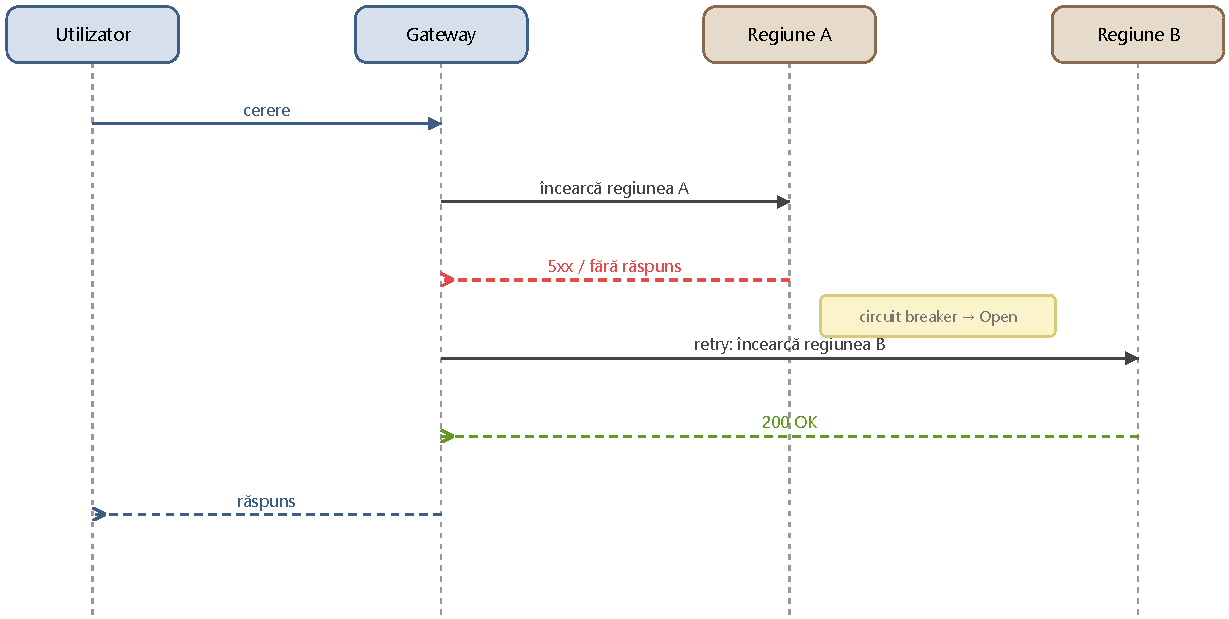
\includegraphics[width=0.92\textwidth]{pics/fig_secventa.pdf}
\caption{Secvența unei cereri cu retry: regiunea preferată răspunde cu eroare, iar gateway-ul face retry al cererii către o regiune funcțională}
\label{fig:seq}
\end{figure}

Atunci când o regiune răspunde cu erori de server sau nu răspunde, load balancer-ul nu propagă eșecul către utilizator, ci face retry al cererii către următoarea regiune din listă. Pentru a evita irosirea de timp pe o regiune defectă, fiecărei perechi serviciu-regiune îi este asociat un mecanism de tip \emph{circuit breaker}~\cite{nygard-circuitbreaker}: după un număr de eșecuri consecutive, regiunea este marcată temporar ca indisponibilă și ocolită, fiind reintrodusă în circuit numai după ce un număr de verificări reușite confirmă revenirea ei. Acest comportament protejează atât utilizatorul, cât și regiunea aflată în dificultate, evitând suprasolicitarea ei. Figura~\ref{fig:cb} prezintă cele trei stări ale acestui mecanism și tranzițiile dintre ele.

\begin{figure}[H]
\centering
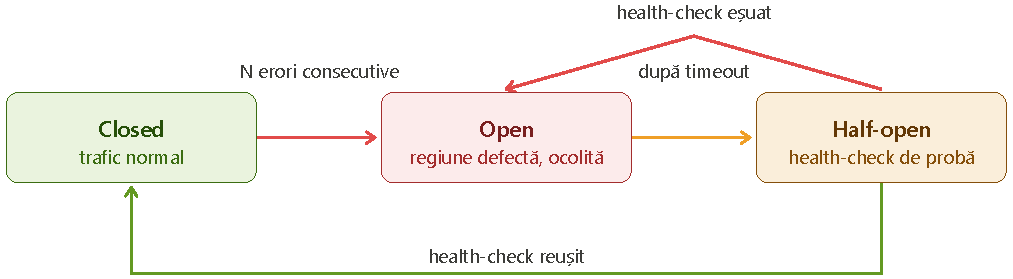
\includegraphics[width=0.88\textwidth]{pics/fig_circuit_breaker.pdf}
\caption{Stările mecanismului circuit breaker asociat fiecărei perechi serviciu-regiune și tranzițiile dintre ele}
\label{fig:cb}
\end{figure}

Configurația care descrie serviciile, path-urile și regiunile lor nu este fixată în cod, ci este preluată periodic din S3 și aplicată la cald. În felul acesta, deciziile luate în consolă se propagă automat către toate gateway-urile, fără repornirea acestora.

\section{Rutarea globală a traficului}
Deasupra gateway-urilor regionale se află stratul de direcționare globală, realizat cu serviciul de \emph{load balancing} al Cloudflare. Fiecărei regiuni îi corespunde un origin pool care indică gateway-ul regional, iar o politică de rutare bazată pe proximitate alege, pentru fiecare utilizator, pool-ul cel mai apropiat geografic. Un health monitor verifică periodic starea fiecărui gateway, iar atunci când regiunea cea mai apropiată devine indisponibilă, traficul este reorientat automat către un pool alternativ.

Astfel, sistemul dispune de două niveluri complementare de reziliență: la nivel global, failover-ul între regiuni realizat de stratul Cloudflare; la nivel regional, retry-ul între regiuni realizat de gateway-ul propriu. Primul nivel reduce latența și tratează defectarea unei întregi regiuni, în timp ce al doilea tratează defecțiunile locale, la nivel de serviciu și de instanță.

\section{Modelul de date și sursa de adevăr}
Starea platformei este păstrată în două mijloace de stocare complementare. DynamoDB este sursa de adevăr pentru starea sistemului: păstrează înregistrările deployment-urilor, împreună cu conturile operatorilor. S3 găzduiește artefactele aplicațiilor și configurația de rutare, câte un fișier diferit pentru fiecare regiune; această configurație este regenerată de consolă din starea deployment-urilor și este citită direct de gateway-uri, fiind sursa de adevăr pentru planul de date.

O aplicație administrată este reprezentată printr-o înregistrare de deployment care reunește identitatea serviciului, regiunea, proprietarul, starea curentă și un inventar al resurselor de infrastructură provizionate pentru ea, alături de evidența pașilor de punere în funcțiune și de deprovizionare. Acest inventar permite consolei să elibereze ulterior, în mod determinist, exact resursele create. Figura~\ref{tab:date} rezumă rolul fiecăruia.

\begin{figure}[H]
\centering
\small\linespread{1.1}
\begin{tabular}{@{}>{\raggedright\arraybackslash}p{3cm}
                   >{\raggedright\arraybackslash}p{4.8cm}
                   >{\raggedright\arraybackslash}p{4.8cm}@{}}
\toprule
\textbf{Stocare} & \textbf{Conținut} & \textbf{Rol} \\
\midrule
DynamoDB & înregistrările deployment-urilor, conturile operatorilor & sursă de adevăr pentru starea sistemului; consultată de consolă \\
\addlinespace
S3 & artefactele aplicațiilor, configurația de rutare pe regiuni & sursă de adevăr pentru planul de date; configurația e citită de gateway-uri \\
\bottomrule
\end{tabular}
\vspace{4pt}
\caption{Stocarea stării platformei}
\label{tab:date}
\end{figure}

% ====================================================================
%  CAPITOLUL 5. DETALII DE IMPLEMENTARE
% ====================================================================
\chapter{Detalii de implementare}

Acest capitol detaliază modul în care a fost realizată platforma, insistând asupra elementelor care au ridicat dificultăți tehnice deosebite. Sunt prezentate, pe rând: organizarea sistemului pe componente, consola de administrare împreună cu pipeline-ul de provizionare și deprovizionare, generarea și distribuția configurației de rutare, încărcarea dinamică a acesteia în load balancer, mecanismul rutării, incluzând și scenariul de failover, mecanismul de circuit breaker împreună cu monitorizarea disponibilității regiunilor, integrarea cu Cloudflare și persistența stării.

\section{Organizarea sistemului}
Platforma este alcătuită din două componente dezvoltate și puse în funcțiune independent. \emph{Consola de administrare} este o aplicație Python/Flask care orchestrează provizionarea și menține starea sistemului. \emph{Load balancer-ul} (gateway-ul) este o aplicație Java construită peste Spring Cloud Gateway, rulată într-un Auto Scaling Group, cu una sau mai multe instanțe în fiecare regiune. Peste aceste componente, operatorul pune în funcțiune serviciile propriu-zise, găzduite tot pe instanțe EC2 grupate în Auto Scaling Group-uri.

Cele trei componente nu comunică direct între ele, ci prin starea partajată din cloud. Consola scrie starea aplicațiilor în DynamoDB și publică în S3 configurația de rutare derivată din ea; fiecare gateway citește din S3 doar configurația propriei regiuni; stratul Cloudflare orientează utilizatorii către gateway-ul cel mai apropiat. Această indirecție menține componentele cuplate slab și permite ca fiecare să funcționeze chiar dacă altele sunt oprite.

Un aspect transversal de implementare este modelul de acces la cloud. Pe infrastructura reală, atât consola, cât și gateway-urile rulează pe instanțe EC2 cărora le este atașat un IAM role; accesul la serviciile AWS se face prin lanțul implicit de credențiale al SDK-ului, fără chei statice în cod sau în artefacte. Același principiu se aplică și la împachetarea consolei pentru deployment: din fișierul de configurație inclus în arhivă, cheile de acces AWS statice sunt eliminate explicit înainte de publicare, întrucât pe instanța EC2 ele sunt furnizate de IAM role.

\section{Consola de administrare}
Consola expune o interfață web prin care operatorul administrează întregul portofoliu: dashboard-uri cu starea aplicațiilor, pentru punerea în funcțiune și extinderea în regiuni, precum și pentru administrarea conturilor. Pe lângă paginile interactive, consola oferă endpoint-uri care declanșează provizionarea și deprovizionarea, fiecare dintre acestea fiind însoțit de un flux de evenimente \emph{server-sent events} prin care progresul este transmis în timp real către browser. Tabloul de bord este prezentat în Figura~\ref{fig:sc-dashboard}.

\begin{figure}[H]
\centering
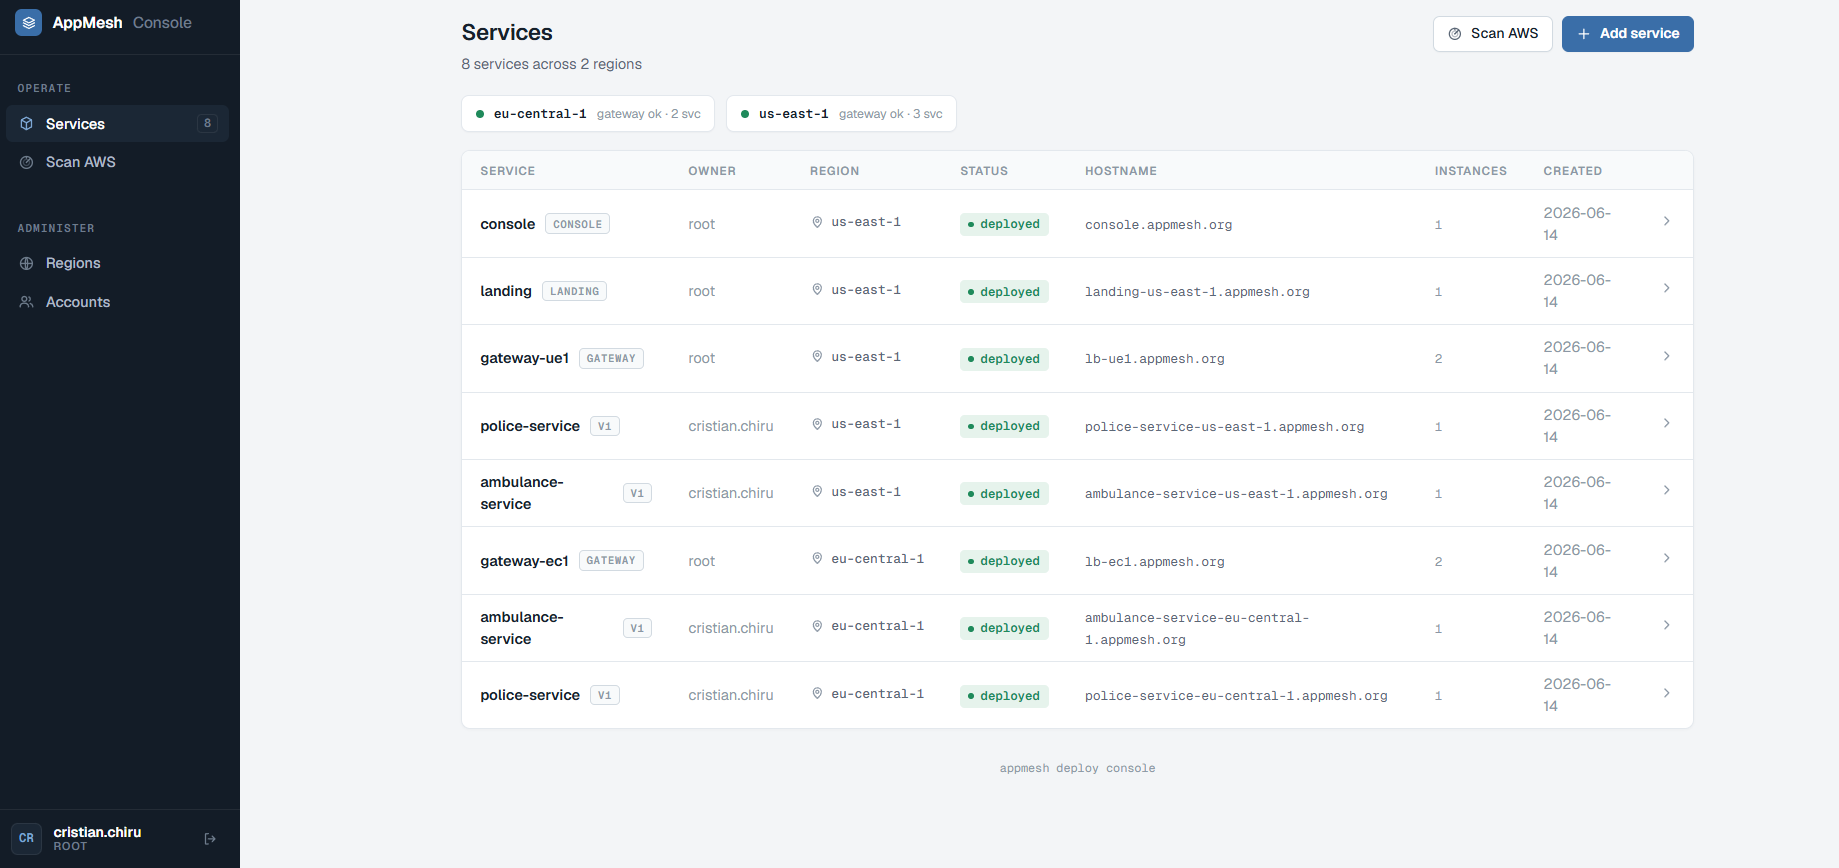
\includegraphics[width=\textwidth]{pics/sc-dashboard.png}
\caption{Tabloul de bord al consolei de administrare}
\label{fig:sc-dashboard}
\end{figure}

Accesul este protejat prin autentificare, cu două roluri: un operator administrator, care gestionează conturile celorlalți, și operatori obișnuiți, care își administrează propriile aplicații. Conturile sunt păstrate în DynamoDB, iar fiecare cerere către consolă trece printr-o verificare de autorizare: un operator obișnuit poate vedea și opera numai deployment-urile al căror proprietar este, în timp ce operațiile la nivel de sistem, precum scanarea întregului cluster sau administrarea conturilor și a regiunilor, sunt rezervate operatorului administrator. Autentificarea se realizează printr-o pagină de login (Figura~\ref{fig:sc-login}), iar conturile operatorilor sunt gestionate dintr-o pagină dedicată, accesibilă doar administratorului (Figura~\ref{fig:sc-accounts}).

\begin{figure}[H]
\centering
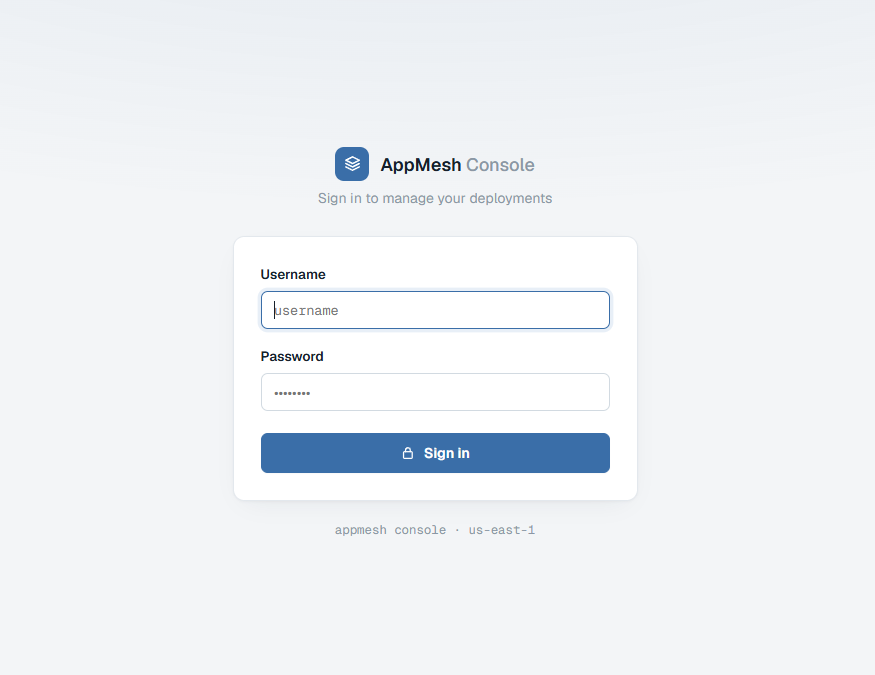
\includegraphics[width=\textwidth]{pics/sc-login.png}
\caption{Pagina de autentificare a consolei}
\label{fig:sc-login}
\end{figure}

\begin{figure}[H]
\centering
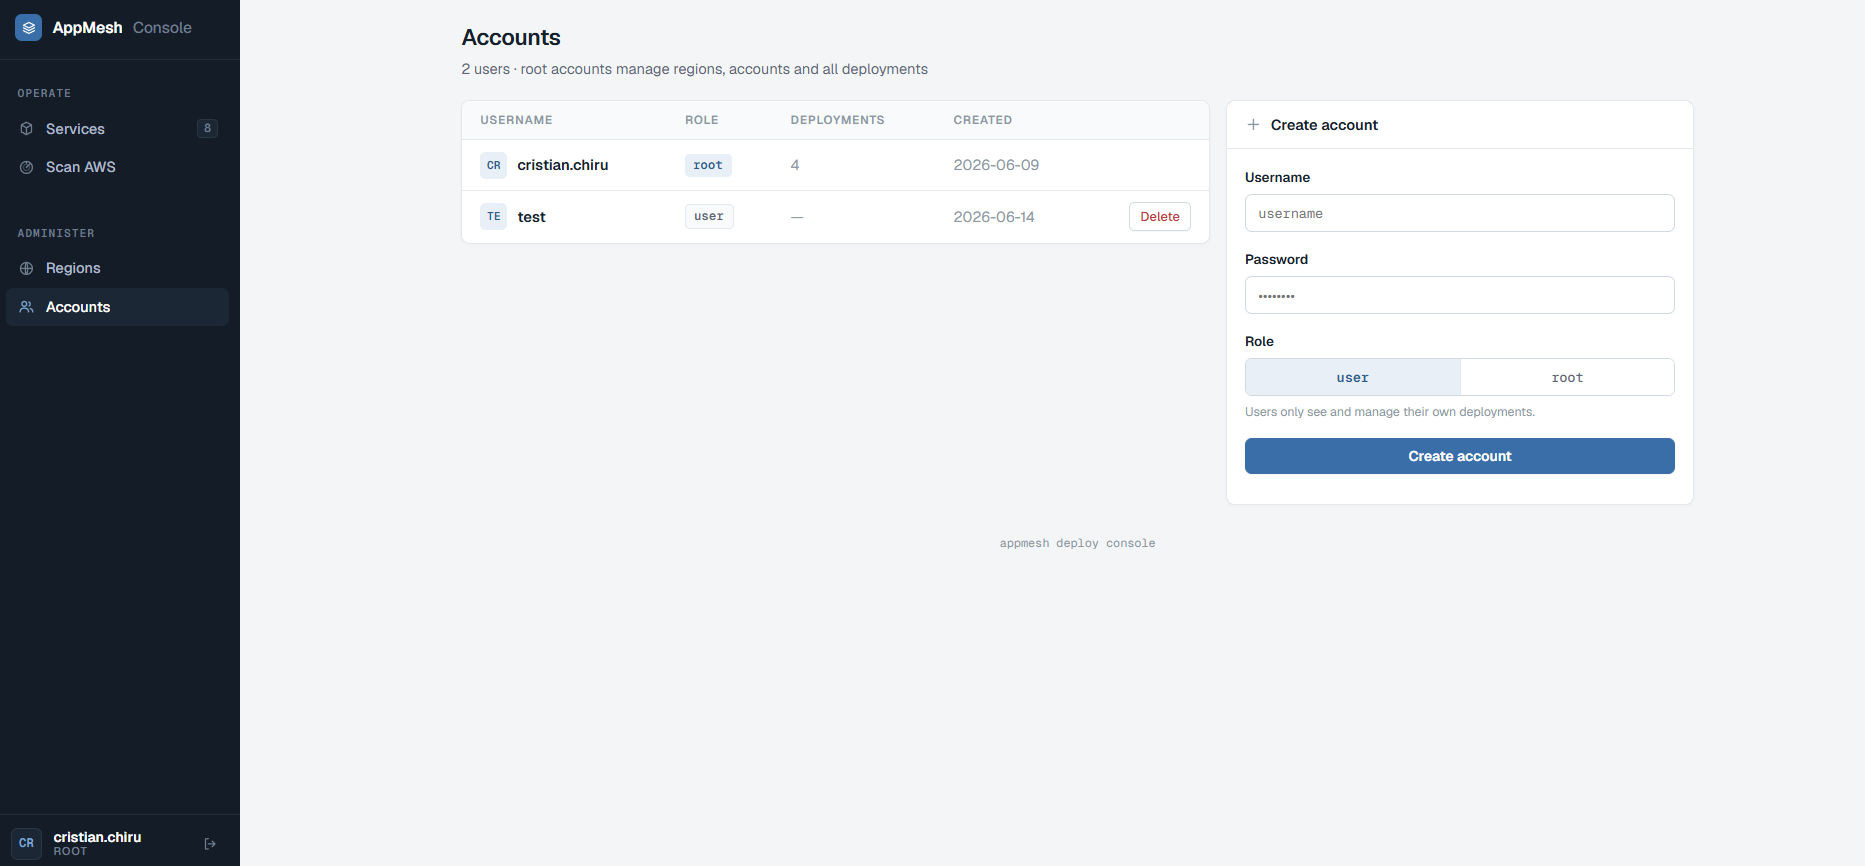
\includegraphics[width=\textwidth]{pics/sc-accounts.png}
\caption{Pagina de administrare a conturilor de operator}
\label{fig:sc-accounts}
\end{figure}

Punerea în funcțiune a unei aplicații pornește dintr-un formular în care operatorul încarcă artefactul aplicației, îi atribuie un nume și alege regiunile în care trebuie să ruleze (Figura~\ref{fig:sc-new}); la trimiterea formularului, consola declanșează provizionarea în fundal.

\begin{figure}[H]
\centering
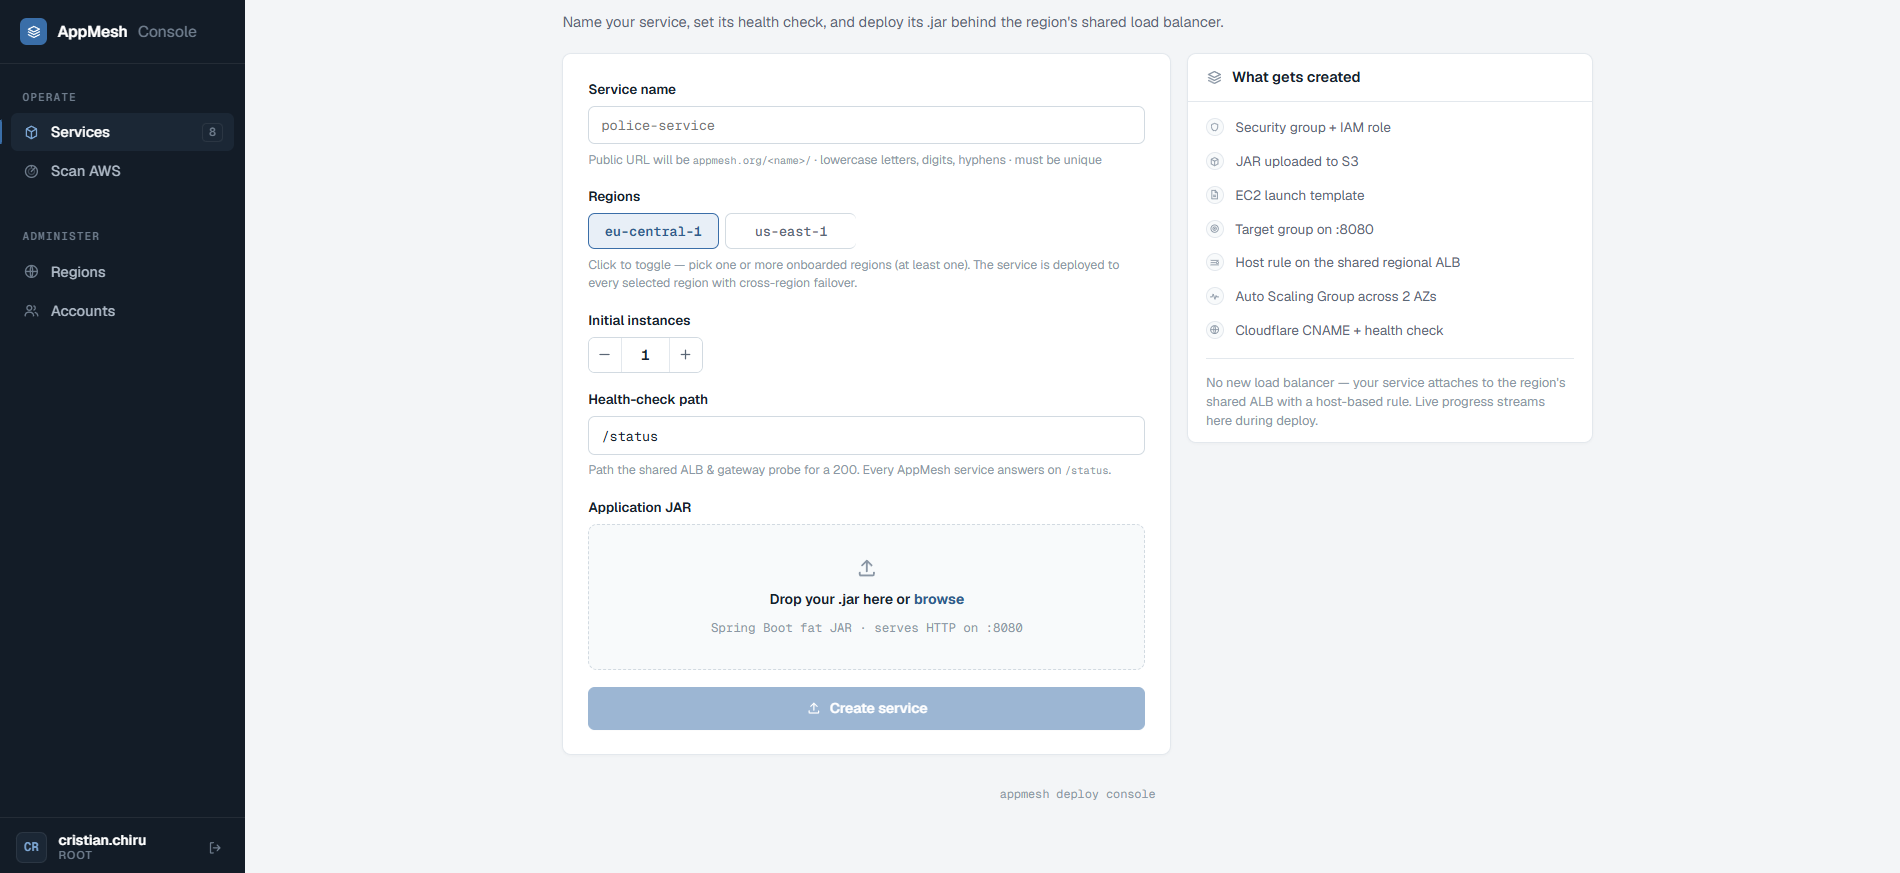
\includegraphics[width=\textwidth]{pics/sc-new.png}
\caption{Formularul de punere în funcțiune a unei aplicații}
\label{fig:sc-new}
\end{figure}

Provizionarea unei aplicații este o operație de durată, așa că este executată într-un fir de execuție separat, în fundal. Pe măsură ce înaintează, fiecare pas actualizează înregistrarea de deployment și incrementează un contor de versiune, pe baza căruia fluxul de evenimente detectează modificările și le transmite interfeței. Operatorul urmărește astfel execuția pas cu pas, cu starea fiecărui pas și eventualele mesaje de eroare. Un exemplu de execuție urmărită în timp real este redat în Figura~\ref{fig:sc-deploy}.

\begin{figure}[H]
\centering
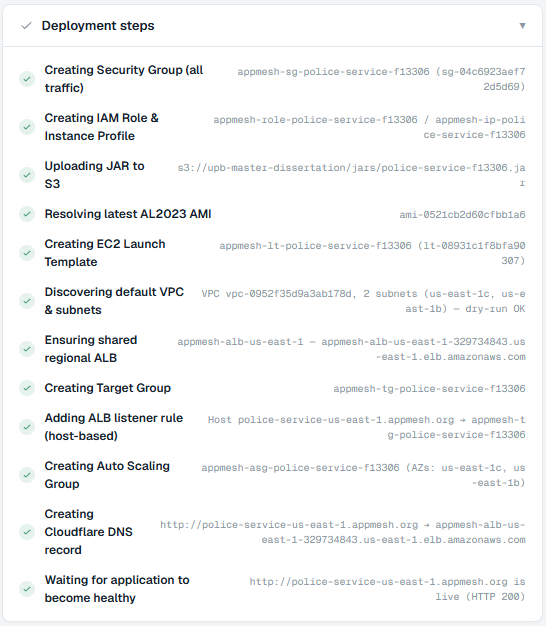
\includegraphics[width=0.42\textwidth]{pics/sc-deploy.png}
\caption{Urmărirea în timp real a provizionării unei aplicații}
\label{fig:sc-deploy}
\end{figure}

Fiecare aplicație din portofoliu are o pagină de detaliu (Figura~\ref{fig:sc-detail}), din care operatorul îi urmărește starea în timp real pe fiecare regiune, îi ajustează numărul de instanțe prin parametrii de auto-scaling și o extinde într-o regiune nouă sau o retrage dintr-una existentă, fără a părăsi contextul serviciului.

\begin{figure}[H]
\centering
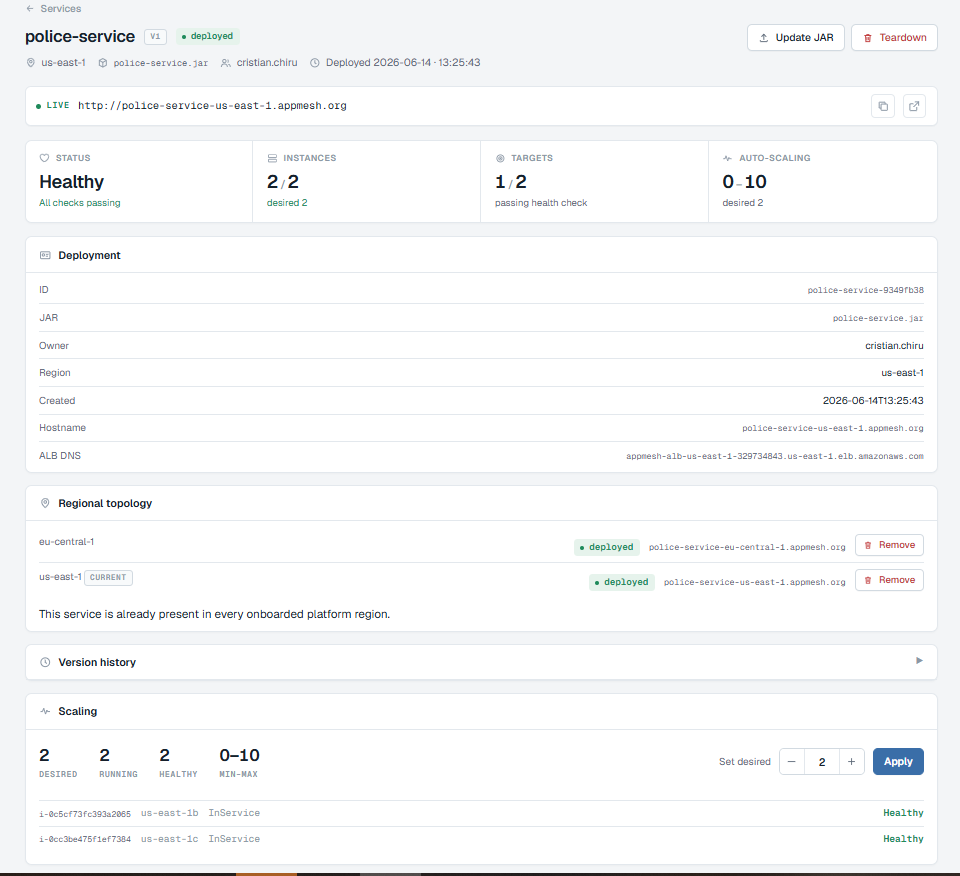
\includegraphics[width=0.92\textwidth]{pics/sc-detail.png}
\caption{Pagina de detaliu a unei aplicații, cu starea pe regiuni și scalarea}
\label{fig:sc-detail}
\end{figure}

Pe lângă administrarea aplicațiilor proprii, consola oferă o funcție de scanare a contului de cloud, prin care resursele AppMesh deja existente sunt descoperite și reconciliate cu evidența internă (Figura~\ref{fig:sc-scan}).

\begin{figure}[H]
\centering
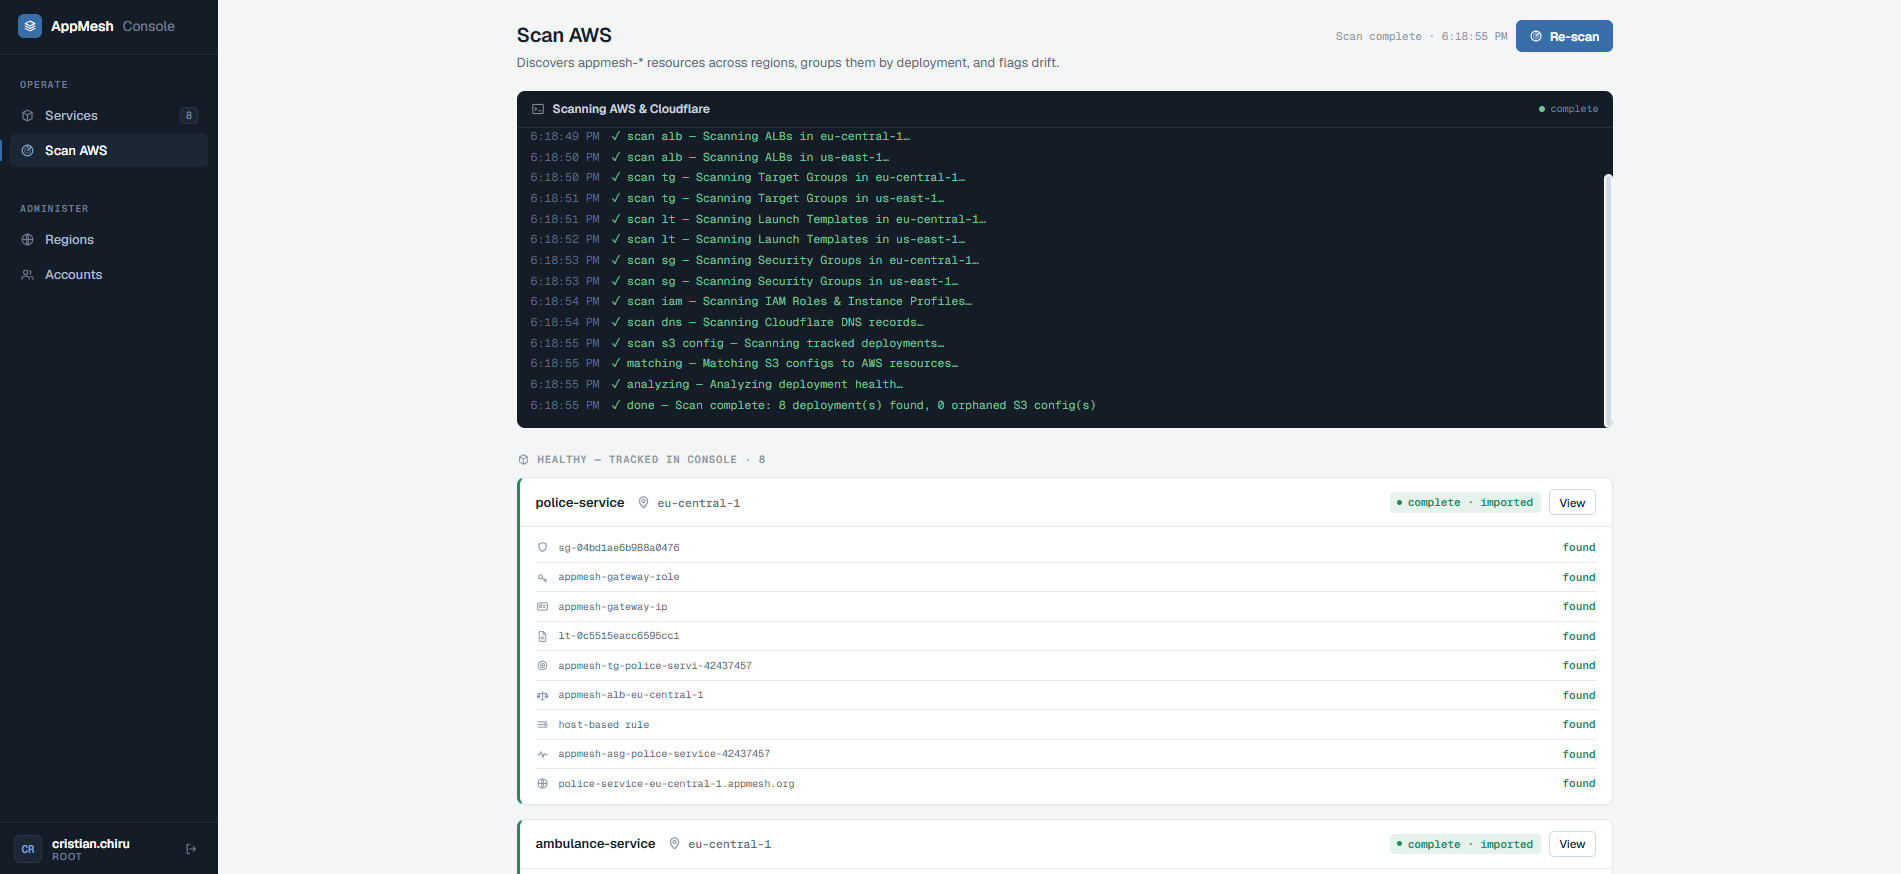
\includegraphics[width=\textwidth]{pics/sc-scan.png}
\caption{Scanarea și reconcilierea resurselor existente în cloud}
\label{fig:sc-scan}
\end{figure}

Aceasta permite preluarea sub administrare a unor deployment-uri create anterior, precum și identificarea resurselor rămase orfane în urma unei operații întrerupte.

\section{Pipeline-ul de provizionare a unei aplicații}
Punerea în funcțiune a unei aplicații parcurge un lanț fix de doisprezece pași, executați în ordine, fiecare provizionând câte o resursă în cloud. Lanțul complet este redat grafic în Figura~\ref{fig:pipeline}.

\begin{figure}[H]
\centering
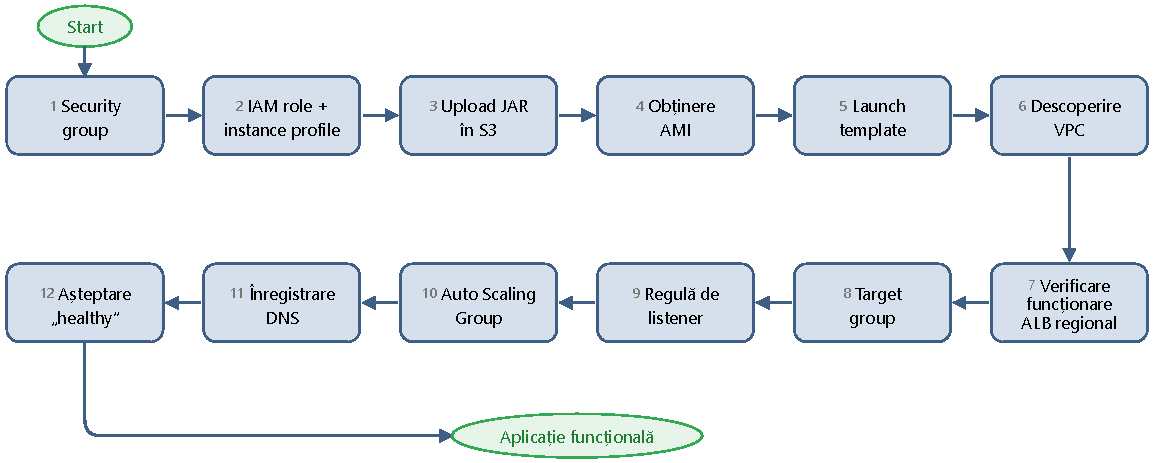
\includegraphics[width=0.97\textwidth]{pics/fig_pipeline.pdf}
\caption{Lanțul de provizionare a unei aplicații: cei doisprezece pași executați în ordine de consolă}
\label{fig:pipeline}
\end{figure}

\needspace{6\baselineskip}
Cei doisprezece pași sunt următorii:

\begin{enumerate}
	\item crearea unui security group care permite traficul către instanțe;
	\item crearea unui IAM role și a instance profile-ului asociat, cu drept de citire din S3;
	\item încărcarea artefactului aplicației în S3;
	\item obținerea celei mai recente imagini AMI Amazon Linux;
	\item crearea unui launch template pentru instanțe;
	\item descoperirea VPC-ului și a subrețelelor implicite;
	\item verificarea prezenței ALB-ului regional partajat în regiune și crearea lui dacă lipsește;
	\item crearea unui target group;
	\item adăugarea unei reguli de listener pe bază de host în ALB;
	\item crearea unui Auto Scaling Group pentru serviciu;
	\item crearea înregistrării DNS în Cloudflare;
	\item așteptarea ca aplicația să devină funcțională.
\end{enumerate}

Fiecare pas își consemnează rezultatul și resursele create într-o înregistrare de deployment, validând totodată efectul produs înainte de a continua. Fragmentul de cod din Figura~\ref{lst:sg} prezintă primul pas, crearea security group-ului și deschiderea traficului de intrare; identificatorul resursei este reținut imediat în deployment, pentru a putea fi eliberat ulterior.

\begin{lstlisting}[language=Python]
sg_id = ec2.create_security_group(
    GroupName=sg_name,
    Description=f"Security group for {dep['name']}",
    VpcId=vpc_id,
)["GroupId"]
ec2.authorize_security_group_ingress(
    GroupId=sg_id,
    IpPermissions=[{
        "IpProtocol": "-1", "FromPort": -1, "ToPort": -1,
        "IpRanges": [{"CidrIp": "0.0.0.0/0"}],
    }],
)
dep["resources"]["security_group_id"] = sg_id
\end{lstlisting}
\captionof{figure}{Crearea security group-ului și a regulii de intrare}\label{lst:sg}

Principala dificultate a acestui lanț a fost eventual consistency a serviciilor AWS. O resursă tocmai creată nu este întotdeauna vizibilă imediat pentru celelalte servicii: în particular, un instance profile nou nu poate fi atașat instantaneu unei instanțe EC2. Pentru a evita eșecul lansării, consola interoghează repetat IAM până când rolul s-a propagat în instance profile, cu o limită de timp, și abia apoi continuă, păstrând și un interval suplimentar de siguranță pentru propagarea între servicii (Figura~\ref{lst:iam}).

\needspace{17\baselineskip}
\begin{lstlisting}[language=Python]
# Un instance profile nou nu este imediat vizibil pentru EC2.
for _ in range(40):
    prof = iam.get_instance_profile(InstanceProfileName=profile_name)
    roles = prof["InstanceProfile"].get("Roles", [])
    if any(r["RoleName"] == role_name for r in roles):
        break
    time.sleep(3)
else:
    raise RuntimeError("instance profile did not propagate after 120s")
time.sleep(15)  # buffer pentru propagarea intre servicii
\end{lstlisting}
\captionof{figure}{Așteptarea propagării instance profile-ului pentru a preveni race condition}\label{lst:iam}

Atunci când o aplicație este pusă în funcțiune în mai multe regiuni, lanțul este executat întâi pentru regiunea primară; după ce aceasta devine funcțională, același artefact deja prezent în S3 este reutilizat pentru a replica serviciul în celelalte regiuni, fără reîncărcare.

Instanțele lansate de Auto Scaling Group nu conțin aplicația preinstalată, ci o obțin la pornire printr-un script de inițializare (user-data), atașat launch template-ului. Scriptul așteaptă serviciul de metadate al instanței, instalează mediul de execuție Java, descarcă artefactul din S3 și înregistrează aplicația ca serviciu \texttt{systemd} cu repornire automată (Figura~\ref{lst:userdata}). În felul acesta, o instanță nou-pornită de scalare automată devine, fără intervenție, un server identic cu celelalte.

\begin{lstlisting}[language=bash]
#!/bin/bash
# Asteapta serviciul de metadate si afla regiunea
TOKEN=$(curl -s -X PUT "http://169.254.169.254/latest/api/token" \
        -H "X-aws-ec2-metadata-token-ttl-seconds: 60")
REGION=$(curl -sf -H "X-aws-ec2-metadata-token: $TOKEN" \
        http://169.254.169.254/latest/meta-data/placement/region)

# Instaleaza mediul de executie si descarca artefactul din S3
dnf -y install java-21-amazon-corretto unzip
aws s3 cp "{s3_uri}" /app/{jar_filename}

# Ruleaza aplicatia ca serviciu systemd, cu repornire automata
cat >/etc/systemd/system/myapp.service <<'EOF'
[Service]
Environment=AWS_REGION={aws_region}
ExecStart=/usr/bin/java -jar /app/{jar_filename}
Restart=always
[Install]
WantedBy=multi-user.target
EOF
systemctl enable myapp && systemctl restart myapp
\end{lstlisting}
\captionof{figure}{Scriptul de inițializare a instanței (user-data)}\label{lst:userdata}

Figura~\ref{fig:topologie} prezintă resursele provizionate pentru un serviciu și relațiile dintre ele.

\begin{figure}[H]
\centering
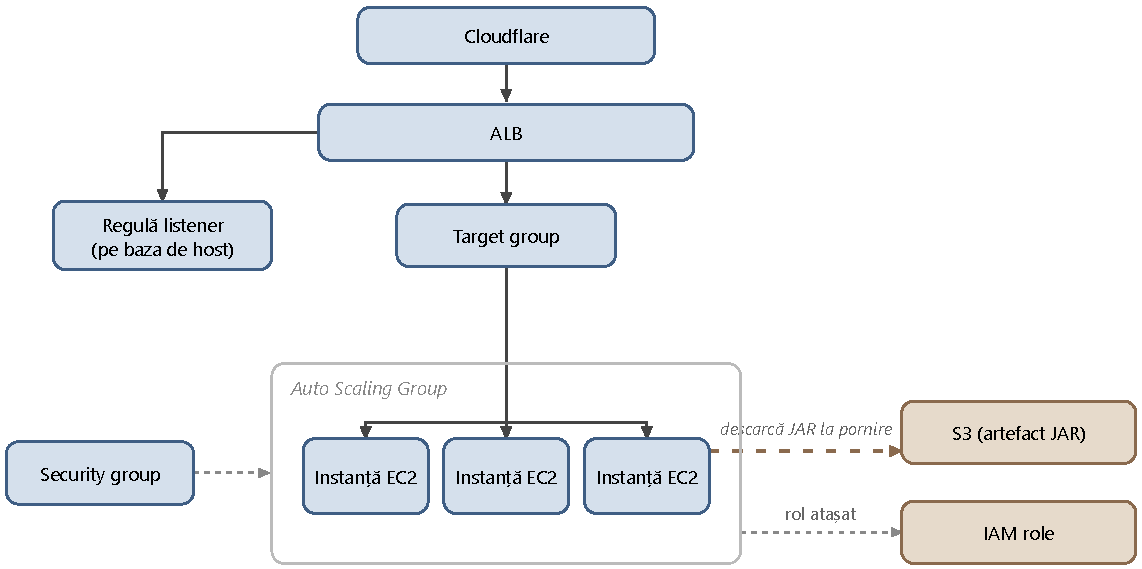
\includegraphics[width=0.92\textwidth]{pics/fig_topologie.pdf}
\caption{Topologia resurselor AWS provizionate pentru un serviciu}
\label{fig:topologie}
\end{figure}

Load balancer-ul regional este partajat: un singur ALB pe regiune deservește, prin reguli de listener pe bază de host, componentele din acea regiune. Această decizie a fost motivată de costurile pentru realizarea prototipului, întrucât fiecare ALB are un cost fix lunar; pentru o implementare mai robustă în producție s-ar separa ingress-ul consolei și al gateway-ului de cel al aplicațiilor, aspect discutat în capitolul de concluzii.

\section{Deprovizionarea resurselor}
Deprovizionarea unei aplicații sau a unei regiuni se sprijină pe resursele consemnate în deployment la provizionare. Pașii sunt parcurși în ordine inversă față de creare, fiindcă resursele depind unele de altele: înregistrarea DNS și Auto Scaling Group-ul sunt eliminate înaintea regulii de listener și a target group-ului; apoi sunt eliminate launch template-ul, instance profile-ul și rolul, artefactul din S3 și, la final, security group-ul. Fiecare ștergere tratează o resursă deja inexistentă ca pe un pas încheiat cu succes și continuă mai departe. Astfel, deprovizionarea este idempotentă și deterministă: elimină exact resursele create, indiferent de punctul în care s-ar fi putut opri o provizionare anterioară, fără a lăsa resurse orfane și fără a atinge resursele partajate, precum ALB-ul regional.

\section{Generarea configurației de rutare}
După fiecare modificare a portofoliului, consola reconstruiește din starea aplicațiilor păstrată în DynamoDB harta serviciilor rutabile. Pentru fiecare serviciu sunt reținute path-urile care îl identifică, path-ul de health-check și lista regiunilor împreună cu adresele lor; gateway-urile și consola, fiind infrastructură, nu sunt rutabile și sunt excluse, iar serviciul de tip landing, pagina din care cetățeanul vede toate serviciile disponibile și alege pe care să îl folosească, este mapat pe path-ul rădăcină. Din această hartă este generat câte un fișier \texttt{application.yml} pentru fiecare regiune activă, publicat în S3 sub o cheie proprie regiunii. Figura~\ref{lst:yaml} arată un astfel de fișier, pentru un serviciu prezent în două regiuni.

\begin{lstlisting}
gateway:
  services:
    police-service:
      paths:
        - /police-service/**
      health-check-path: /status
      regions:
        - name: us-east-1
          url: http://police-service.us-east-1.appmesh.org
        - name: eu-central-1
          url: http://police-service.eu-central-1.appmesh.org
  circuit-breaker:
    failure-threshold: 3
    success-threshold: 2
    half-open-delay-seconds: 30
  health-check:
    interval-seconds: 15
    timeout-seconds: 5
  timeout:
    connect-timeout-ms: 2000
    read-timeout-ms: 5000
\end{lstlisting}
\captionof{figure}{Configurația de rutare generată pentru o regiune (\texttt{application.yml})}\label{lst:yaml}

În fișierul fiecărei regiuni, ordinea regiunilor unui serviciu este rearanjată astfel încât regiunea locală a gateway-ului să apară prima, ceea ce face ca traficul să fie deservit preferențial local. Secțiunea de parametri ai circuit breaker-ului este emisă numai atunci când cel puțin un serviciu este prezent în mai multe regiuni, deoarece pentru serviciile dintr-o singură regiune mecanismul nu are sens.

\section{Încărcarea dinamică a configurației în gateway}
Distribuția configurației către load balancere se face fără repornirea acestora. Fiecare gateway își rezolvă, pe baza regiunii proprii, cheia obiectului care îl privește și interoghează periodic, la cel mult treizeci de secunde, exclusiv acel obiect din S3. O comparație de ETag evită descărcarea atunci când configurația nu s-a schimbat; la o modificare reală, structura de configurație din memorie este repopulată pe loc, iar un eveniment intern de reîmprospătare determină reconstruirea tabelei de rute (Figura~\ref{lst:reload}). Pentru orice eroare la încărcare, gateway-ul păstrează ultima configurație validă și continuă să deservească traficul.

\needspace{18\baselineskip}
\begin{lstlisting}[language=Java]
private synchronized void refresh(String trigger) {
    HeadObjectResponse head = s3.headObject(b -> b.bucket(bucket).key(key));
    String etag = head.eTag();
    if (etag != null && etag.equals(lastEtag)) {
        return;                       // configuratia nu s-a schimbat
    }
    ResponseBytes<GetObjectResponse> obj =
            s3.getObjectAsBytes(b -> b.bucket(bucket).key(key));
    GatewayServicesProperties parsed = parse(obj.asByteArray());
    apply(parsed);                    // repopuleaza bean-ul in loc
    lastEtag = etag;
    events.publishEvent(new RefreshRoutesEvent(this));  // reconstruieste rutele
}
\end{lstlisting}
\captionof{figure}{Reîncărcarea configurației din S3, condiționată de ETag}\label{lst:reload}

\section{Construirea dinamică a rutelor}
Tabela de rute a gateway-ului este construită din configurația încărcată: pentru fiecare serviciu se creează o rută care se potrivește pe path-urile acelui serviciu și căreia i se atașează filtrul ce realizează selecția regiunii și retry-ul. În mod normal, Spring Cloud Gateway ar prelua singur cererea după potrivirea rutei și ar trimite-o către adresa (\texttt{uri}) configurată pe rută. Aici nu se dorește acest comportament implicit, deoarece alegerea regiunii și retry-ul sunt realizate de filtrul propriu; de aceea rutei i se dă o adresă fictivă (\texttt{no://op}) și cererea este marcată ca deja rutată, astfel încât proxy-ul implicit să fie ocolit și întreaga logică să rămână în filtru (Figura~\ref{lst:routes}). Pentru că metoda citește configurația live din memorie, la fiecare eveniment de reîmprospătare tabela de rute este reconstruită automat, reflectând noua topologie a serviciilor.

\begin{lstlisting}[language=Java]
public Flux<Route> getRoutes() {
    RouteLocatorBuilder.Builder routes = builder.routes();
    properties.getServices().forEach((name, svc) -> {
        MultiRegionRouteFilter filter =
                new MultiRegionRouteFilter(name, properties, circuitBreaker);
        routes.route(name, r -> r
                .path(svc.getPaths().toArray(new String[0]))
                .filters(f -> f.filter(filter))
                .uri("no://op"));     // proxy implicit ocolit
    });
    return routes.build().getRoutes();
}
\end{lstlisting}
\captionof{figure}{Construirea unei rute per serviciu, cu filtrul de retry}\label{lst:routes}

\section{Rutarea cu retry}
Pentru fiecare cerere, filtrul îndepărtează prefixul de path corespunzător serviciului, ordonează regiunile punând prima regiunea locală și le încearcă pe rând. O regiune care răspunde cu o eroare de server sau care nu răspunde este înregistrată ca eșec, iar pentru cerere se face retry către următoarea regiune, fără ca utilizatorul să observe; un răspuns de succes este transmis înapoi în flux, în timp ce o eroare de client este considerată problema apelantului, nu a regiunii. Fluxul corespunzător este cel ilustrat în Figura~\ref{fig:seq}, iar Figura~\ref{lst:failover} arată mecanismul deciziei de retry.

\begin{lstlisting}[language=Java]
return requestSpec.exchangeToMono(resp -> {
    if (multiRegion && resp.statusCode().is5xxServerError()) {
        circuitBreaker.recordFailure(cbKey);
        return resp.releaseBody()
                   .then(Mono.error(new RegionFailedException(cbKey)));
    }
    if (multiRegion) circuitBreaker.recordSuccess(cbKey);
    return writeProxiedResponse(exchange, resp);            // succes
}).onErrorResume(ex -> {
    if (!multiRegion) return writeError(exchange, 503, "...");
    return tryRegion(exchange, regions, path, query,
                     method, headers, body, attempt + 1);   // retry
});
\end{lstlisting}
\captionof{figure}{Mecanismul deciziei de retry pentru o regiune}\label{lst:failover}

O dificultate specifică modelului reactiv, neblocant, pe care este construit gateway-ul, este că un corp de cerere poate fi citit o singură dată. Pentru a putea trimite aceeași cerere către o altă regiune, corpul este memorat în prealabil într-un buffer și reutilizat la fiecare retry; fără această precauție, un al doilea apel ar trimite un corp gol. Tot pentru a evita un cost inutil, pentru serviciile prezente într-o singură regiune întregul mecanism de circuit breaker este ocolit, cererea fiind transmisă direct singurului backend.

\section{Mecanismul de circuit breaker}
Fiecărei perechi serviciu-regiune îi este asociată o stare de circuit breaker, cu cele trei stări și tranzițiile descrise în Figura~\ref{fig:cb}. Trecerea din \emph{Closed} în \emph{Open} are loc după trei eșecuri consecutive; după treizeci de secunde, la prima cerere, starea devine \emph{Half-Open}, iar două probe reușite o readuc în \emph{Closed}, în timp ce o singură probă eșuată o trimite înapoi în \emph{Open}. Starea fiecărei chei este protejată împotriva accesului concurent, întrucât mai multe cereri pot fi deservite simultan. Figura~\ref{lst:cb} arată decizia de permitere a unei cereri și înregistrarea unui eșec.

\needspace{30\baselineskip}
\begin{lstlisting}[language=Java]
public boolean isCallPermitted(String key) {
    CBState s = states.computeIfAbsent(key, k -> new CBState());
    synchronized (s) {
        switch (s.state) {
            case CLOSED:    return true;
            case HALF_OPEN: return true;
            case OPEN:
                if (elapsedSince(s.lastFailureTime) > halfOpenDelay) {
                    s.state = State.HALF_OPEN;   // OPEN -> HALF_OPEN
                    return true;
                }
                return false;                    // regiune ocolita
        }
    }
}

public void recordFailure(String key) {
    CBState s = states.get(key);
    synchronized (s) {
        s.failureCount++;
        if (s.state == State.HALF_OPEN
                || s.failureCount >= failureThreshold) {
            s.state = State.OPEN;                // -> OPEN
            s.failureCount = 0;
        }
    }
}
\end{lstlisting}
\captionof{figure}{Permiterea cererilor și deschiderea circuitului}\label{lst:cb}

\section{Monitorizarea activă a sănătății}
Starea circuit breaker-ului este alimentată din două surse complementare. Prima este calea cererii reale: filtrul de rutare înregistrează fiecare succes sau eșec observat la deservirea traficului. A doua este un monitor activ care, independent de trafic, interoghează la fiecare cincisprezece secunde path-ul de health-check al fiecărei regiuni a fiecărui serviciu prezent în mai multe regiuni și transmite rezultatul aceluiași mecanism de circuit breaker. Datorită acestei a doua surse, o regiune defectă este ocolită rapid, iar revenirea ei este detectată automat, prin probele de health-check, chiar și în absența traficului real care ar fi declanșat altfel tranziția înapoi în \emph{Closed}.

\section{Rutarea globală cu Cloudflare}
La nivel global, fiecărei regiuni îi corespunde un origin pool care indică gateway-ul ei, cu coordonatele geografice ale regiunii și cu un health monitor atașat. Deasupra lor, un load balancer pe domeniul \texttt{appmesh.org} folosește o politică de rutare bazată pe proximitate pentru a orienta fiecare utilizator către pool-ul cel mai apropiat și comută automat traficul către un pool alternativ atunci când regiunea preferată devine indisponibilă (Figura~\ref{lst:cf}). Configurația acestui strat este gestionată tot de consolă. Întrucât planul Cloudflare folosit în dezvoltare permite doar un număr fix de origin pool-uri, anume două, stratul global a fost limitat la două regiuni; scalarea la mai multe ar necesita un plan superior.

\begin{lstlisting}[language=Python]
def _cf_apex_lb_payload(pool_ids):
    return {
        "name": CF_LB_NAME,                 # appmesh.org
        "proxied": True,
        "steering_policy": "proximity",     # cel mai apropiat pool
        "default_pools": pool_ids,
        "fallback_pool": pool_ids[0],
        "location_strategy": {"mode": "pop", "prefer_ecs": "proximity"},
        "adaptive_routing": {"failover_across_pools": True},
    }
\end{lstlisting}
\captionof{figure}{Configurația load balancer-ului Cloudflare}\label{lst:cf}

Acest strat se suprapune peste retry-ul intern al gateway-ului, rezultând două niveluri complementare de reziliență: cel global, prin failover între regiuni la nivel de Cloudflare, tratează defectarea unei întregi regiuni, apropiind în același timp serviciul de utilizatori, iar cel intern tratează defecțiunile locale, la nivel de serviciu și de instanță.

\section{Aplicațiile demonstrative}
Pentru a valida platforma au fost realizate două servicii guvernamentale demonstrative, unul de ambulanță și unul de poliție, ca aplicații Spring Boot. Rolul lor nu este să implementeze o logică de afaceri reală, ci să facă vizibil comportamentul platformei: fiecare instanță își află, la pornire, regiunea și identificatorul propriu, interogând serviciul de metadate al instanței EC2, și le expune în răspunsuri.

Fiecare instanță își expune regiunea și identitatea atât într-o pagină de prezentare lizibilă, cât și într-un răspuns structurat. Reîmprospătând pagina de prezentare în timpul unei defecțiuni, se poate observa direct cum regiunea care răspunde se schimbă atunci când intervine retry-ul gateway-ului, ceea ce transformă un mecanism intern, altfel invizibil, într-un comportament observabil, util pentru demonstrarea soluției. Paginile de prezentare ale celor două servicii demonstrative sunt redate în Figura~\ref{fig:sc-welcome}, fiecare afișând în colțul din dreapta sus versiunea, instanța și regiunea care o deservesc.

\begin{figure}[H]
\centering
\centerline{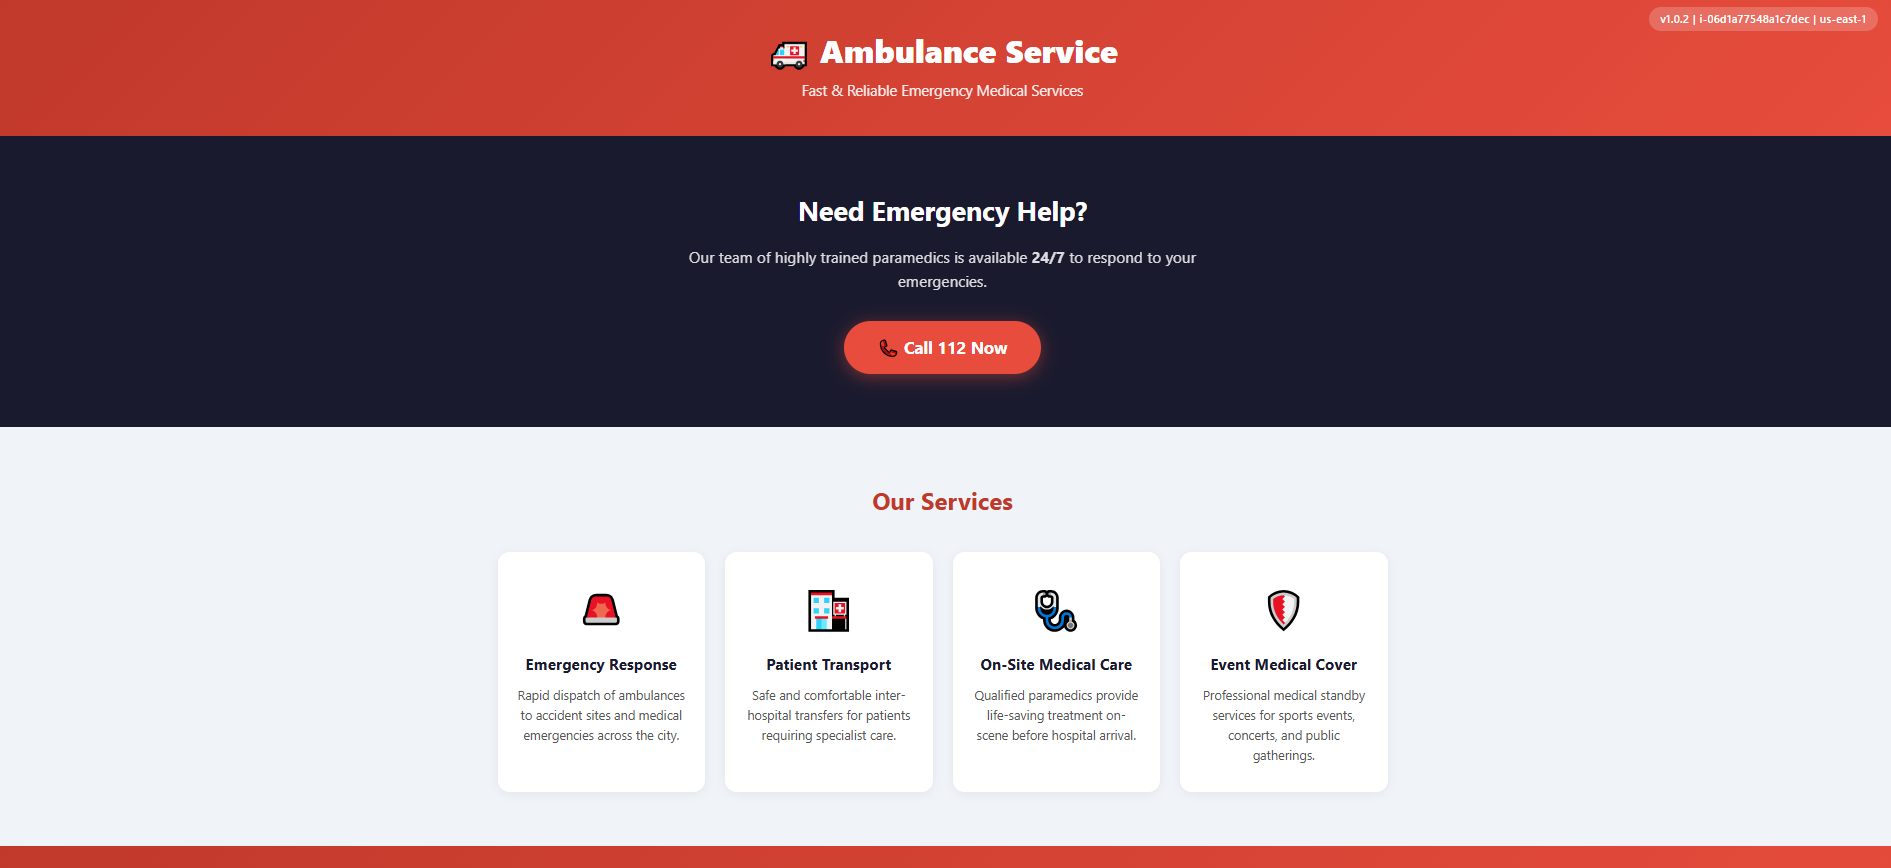
\includegraphics[width=0.8\textwidth]{pics/sc-welcome-ambulance.png}}
\vspace{10pt}
\centerline{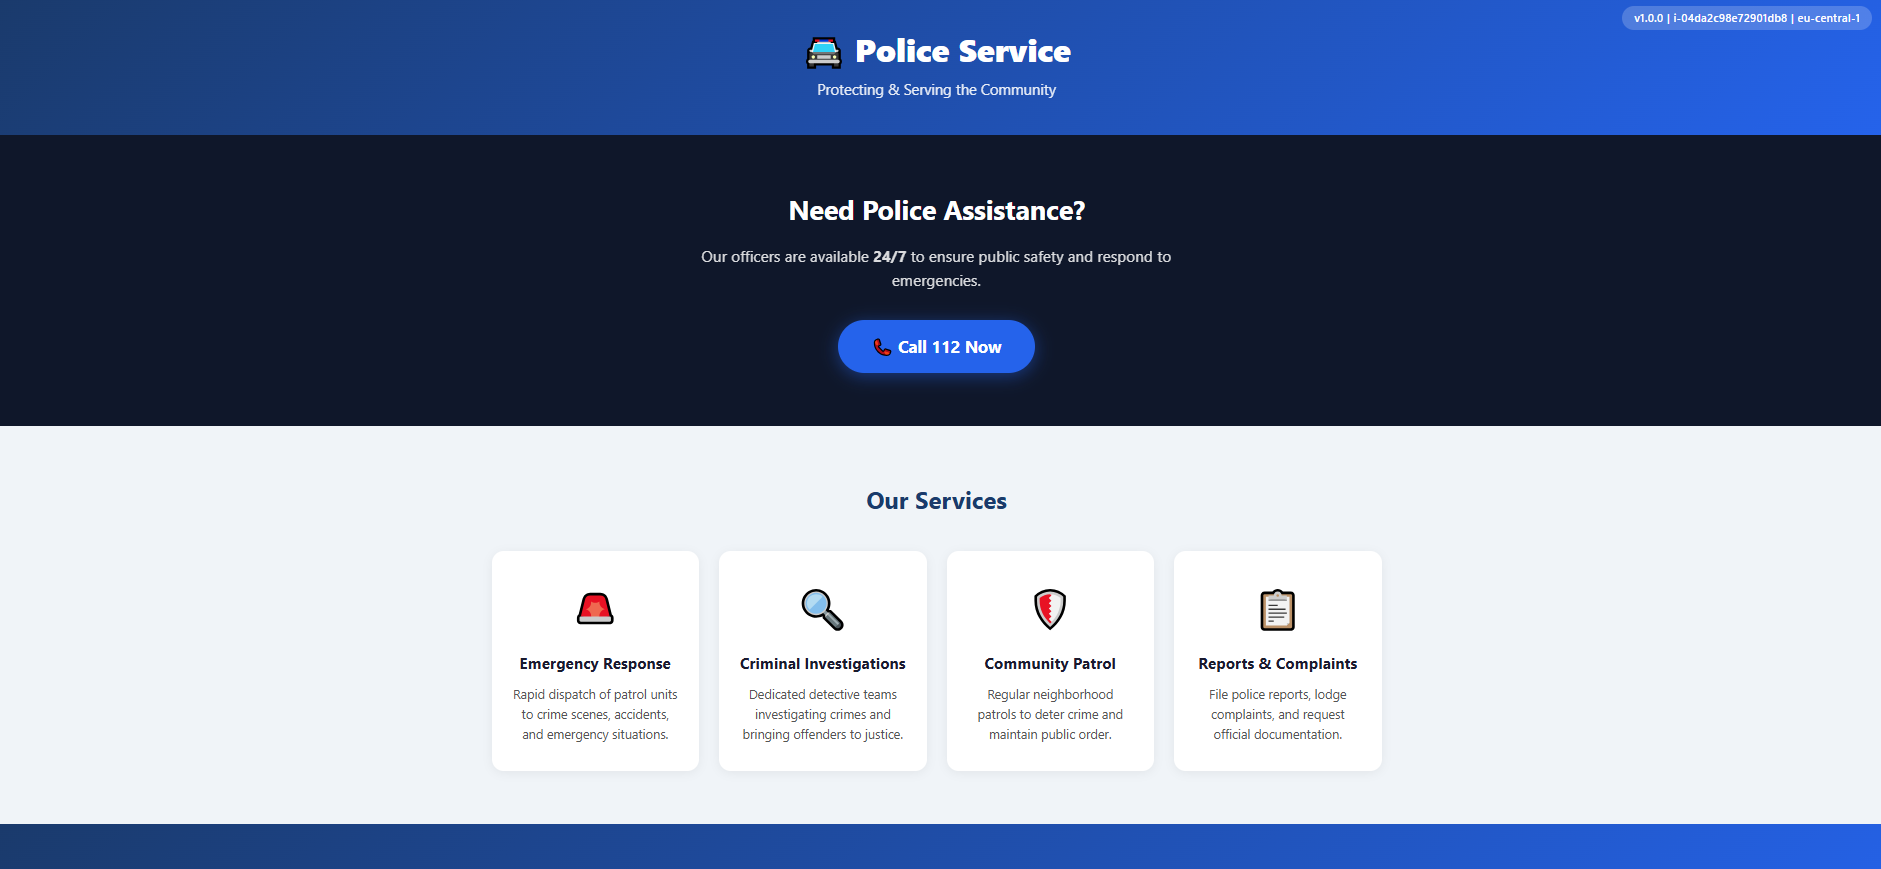
\includegraphics[width=0.8\textwidth]{pics/sc-welcome-police.png}}
\caption{Paginile de prezentare ale celor două servicii demonstrative, ambulanță (sus) și poliție (jos), fiecare cu regiunea și instanța care răspund}
\label{fig:sc-welcome}
\end{figure}

Aceleași informații sunt expuse programatic de un endpoint \texttt{/status}, folosit drept path de health-check atât de load balancer-ul regional, cât și de gateway, care întoarce starea împreună cu regiunea și instanța care deservesc cererea (Figura~\ref{lst:status}).

\begin{lstlisting}[language=Java]
@GetMapping("/status")
@ResponseBody
public ResponseEntity<Map<String, String>> status() {
    return ResponseEntity.ok(Map.of(
            "status", "UP",
            "version", version,
            "instanceId", instanceId,   // citite la pornire din
            "region", region            // serviciul de metadate EC2
    ));
}
\end{lstlisting}
\captionof{figure}{Endpoint-ul de health-check care expune regiunea și instanța}\label{lst:status}

Pe lângă paginile serviciilor individuale, platforma expune o pagină de tip landing, mapată pe path-ul rădăcină, din care cetățeanul vede toate serviciile guvernamentale disponibile și alege pe care să îl acceseze (Figura~\ref{fig:sc-landing}).

\begin{figure}[H]
\centering
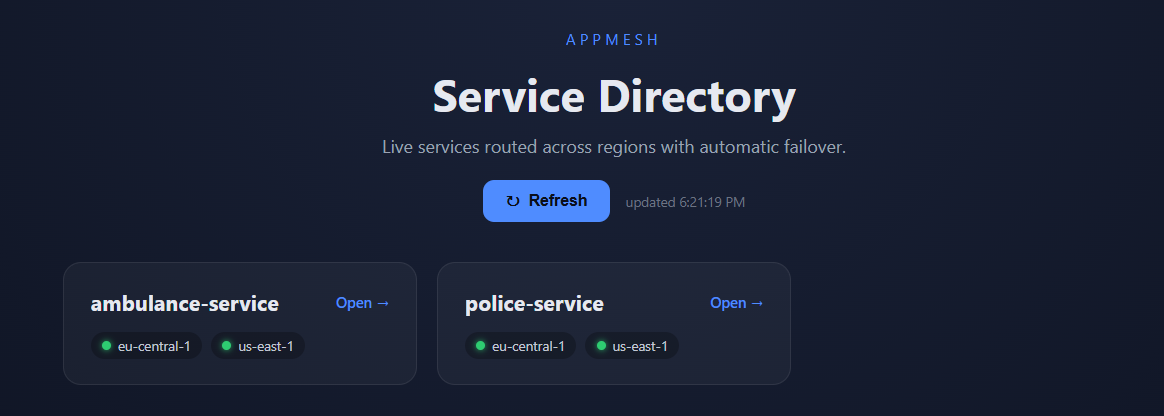
\includegraphics[width=\textwidth]{pics/sc-landing.png}
\caption{Pagina de tip landing, cu serviciile disponibile pentru cetățean}
\label{fig:sc-landing}
\end{figure}

\section{Persistența stării}
Starea platformei este distribuită între DynamoDB și S3, cu roluri complementare. În DynamoDB sunt două tabele: una pentru conturile operatorilor și una pentru deployment-uri. O înregistrare de deployment reunește identitatea serviciului, regiunea, proprietarul, starea curentă, evidența resurselor de infrastructură provizionate și istoricul pașilor de provizionare și de deprovizionare; conținutul detaliat este serializat ca document, alături de câmpurile după care se fac interogările. În S3 sunt păstrate artefactele aplicațiilor și fișierele de configurație de rutare, câte unul pentru fiecare regiune. Această împărțire reflectă cele două roluri: DynamoDB este sursa de adevăr pentru starea sistemului, consultată de consolă, iar S3 este sursa de adevăr pentru planul de date, citită de gateway-uri. Evidența resurselor provizionate, păstrată în înregistrarea de deployment, este cea care face posibilă deprovizionarea deterministă descrisă mai sus.

% ====================================================================
%  CAPITOLUL 6. TESTARE SI VALIDARE
% ====================================================================
\chapter{Testare și validare}

Validarea unei platforme care orchestrează infrastructură reală în cloud ridică o dificultate aparte: corectitudinea nu poate fi judecată după ceea ce raportează consola despre sine, ci după efectul produs efectiv asupra resurselor din cloud. Din acest motiv, platforma a fost verificată printr-o suită automată care verifică sistemul în întregime, de la cererea trimisă consolei până la resursele provizionate, și care confirmă fiecare efect independent de consolă. Acest capitol descrie strategia și metodologia de testare, trasabilitatea față de cerințe, rezultatele obținute și defectele identificate și remediate, încheind cu scenariul de failover indus, care validează comportamentul central al platformei.

\section{Strategia de testare}
Suita de testare este scrisă în Python și verifică o instanță reală a consolei, pornită local și conectată la conturi reale de AWS și Cloudflare. Testarea se face la nivelul interfeței expuse de consolă, tratând-o ca pe o cutie neagră: fiecare scenariu trimite cereri HTTP către endpoint-urile publice, exact cum ar face un operator, și observă apoi rezultatul. Spre deosebire de un test unitar clasic, accentul nu cade pe funcții izolate, ci pe comportamentul întregului sistem în condiții cât mai apropiate de cele de producție.

Suita este organizată într-o bibliotecă de utilitare comune și patru fișiere, câte unul pentru fiecare fază. Biblioteca oferă un client de consolă cu sesiune persistentă, funcții de așteptare a stărilor de durată (provizionare, deprovizionare, scalare) și un mecanism uniform de raportare a verificărilor, în care fiecare aserțiune este marcată ca reușită sau eșuată și agregată într-un rezumat final. În total, cele patru faze însumează peste o sută treizeci de verificări individuale.

O parte din scenarii sunt nedistructive, în sensul că nu provizionează resurse în cloud, ci doar verifică logica de autentificare, autorizare, validare a intrărilor și tratare a erorilor; restul scenariilor parcurg ciclul complet de viață al unei aplicații și, prin urmare, creează și eliberează resurse reale. Această separare permite rularea rapidă și repetată a verificărilor funcționale, fără costul și durata unei provizionări complete.

\section{Metodologia în patru faze}
Testarea este structurată în patru faze, fiecare construind pe stabilitatea confirmată de cea anterioară:

\begin{itemize}
	\item \textbf{Faza 1, funcțional și cazuri-limită}, vizează consola fără a proviziona resurse. Sunt verificate accesul la endpoint-urile publice și redirecționarea celor protejate, autentificarea cu credențiale corecte și greșite, restricționarea operațiilor la nivel de sistem doar pentru operatorul administrator, gestionarea conturilor, izolarea între operatori (un operator nu vede și nu poate acționa asupra resurselor altuia), validarea formularului de punere în funcțiune (artefact lipsă sau de tip greșit, nume invalid, regiune neonboardată, număr negativ de instanțe) și tratarea cererilor eronate.
	\item \textbf{Faza 2, ciclul de viață într-o singură regiune}, pune efectiv în funcțiune un serviciu și îi parcurge întreaga viață: provizionarea cu verificarea fiecărei resurse, scalarea de la o instanță la trei și înapoi, actualizarea artefactului cu incrementarea versiunii și, în final, deprovizionarea cu eliberarea tuturor resurselor. Fiecare etapă este urmată de o comparare a stării observate în cloud cu cea așteptată.
	\item \textbf{Faza 3, persistență și reziliență}, verifică faptul că operațiile de durată supraviețuiesc evenimentelor neprevăzute. Sunt testate trei situații: o deprovizionare aflată în curs continuă corect după ce operatorul se deconectează și se reconectează; o deprovizionare întreruptă de oprirea bruscă a consolei este reluată automat la repornire, sărind peste pașii deja încheiați; iar o provizionare întreruptă în același mod este anulată prin rollback, fără a lăsa resurse orfane.
	\item \textbf{Faza 4, multi-region și failover}, este cea mai complexă. Ea adaugă o a doua regiune, pune în funcțiune același serviciu în ambele, verifică rutarea pe baza path-ului prin gateway, induce apoi o defecțiune și observă failover-ul, după care elimină regiunea adăugată și readuce platforma la starea de bază. Tot aici este confirmată aplicarea configurărilor în Cloudflare: crearea origin pool-ului pentru noua regiune și includerea lui în load balancer-ul global.
\end{itemize}

Cele patru faze și ordinea lor sunt rezumate în Figura~\ref{fig:qafaze}.

\begin{figure}[H]
\centering
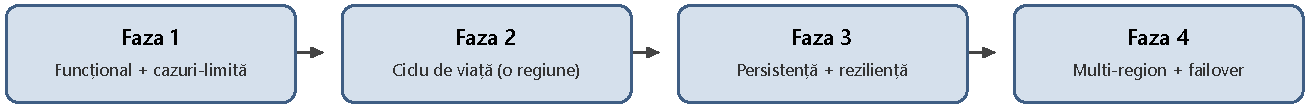
\includegraphics[width=0.98\textwidth]{pics/fig_qa_faze.pdf}
\caption{Cele patru faze ale suitei de testare, în ordinea creșterii complexității și a impactului asupra infrastructurii}
\label{fig:qafaze}
\end{figure}

Pagina de administrare a regiunilor, prin care faza a patra adaugă și elimină regiuni, este prezentată în Figura~\ref{fig:sc-regions}.

\begin{figure}[H]
\centering
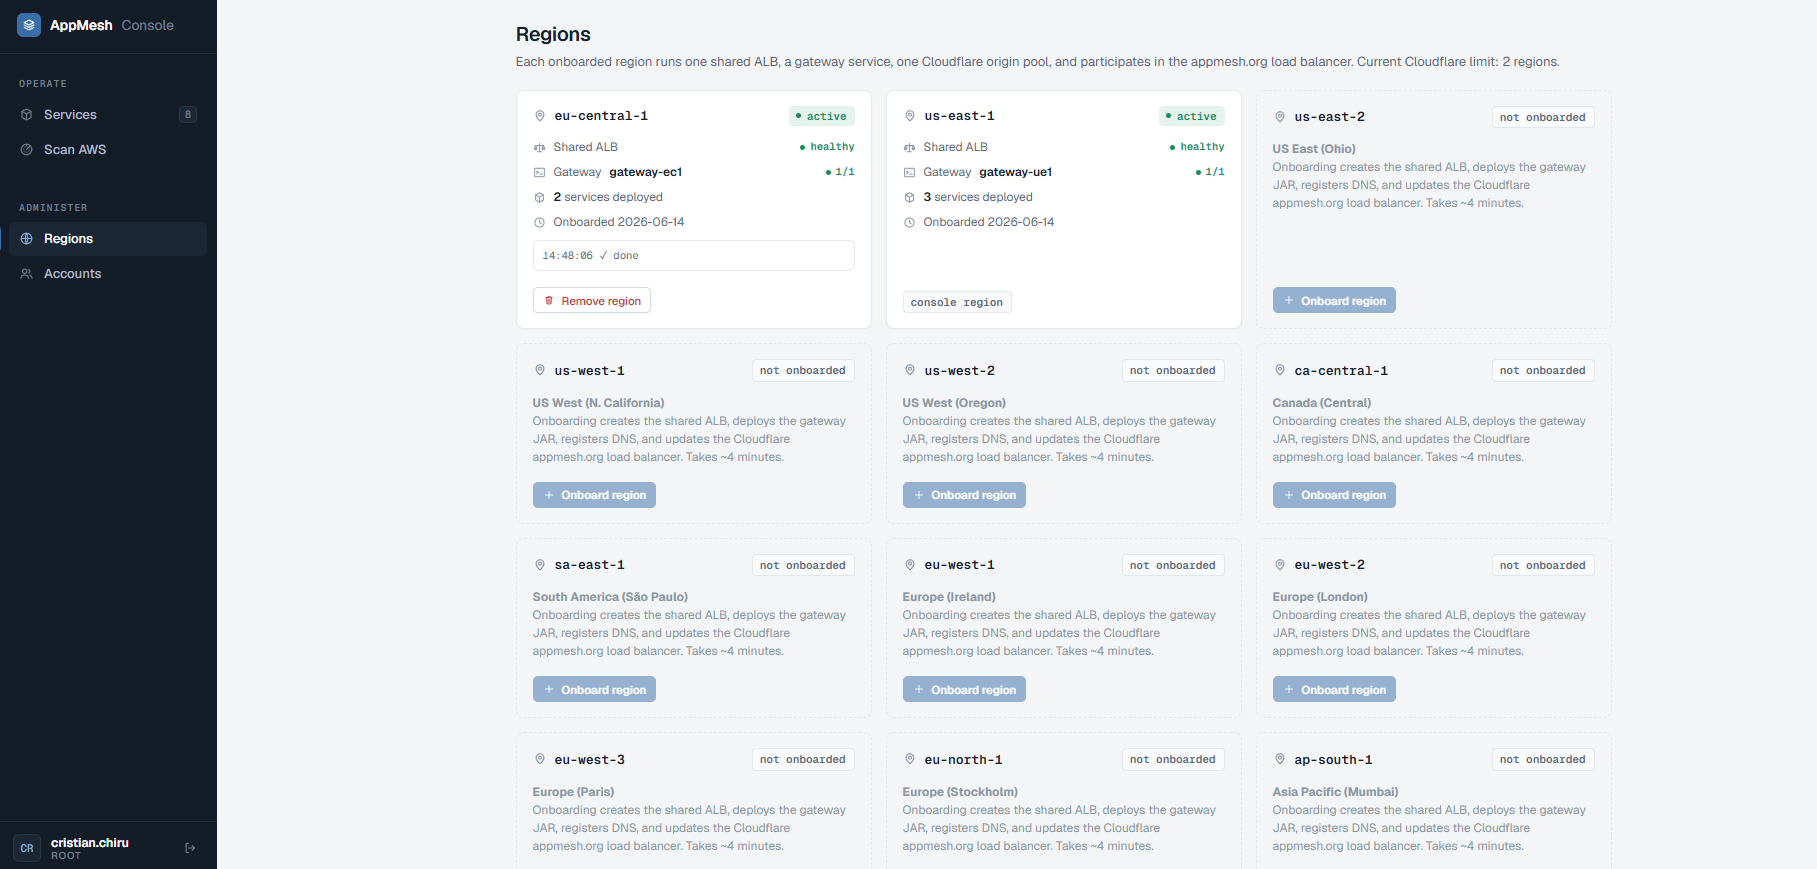
\includegraphics[width=\textwidth]{pics/sc-regions.png}
\caption{Pagina de administrare a regiunilor active}
\label{fig:sc-regions}
\end{figure}

\section{Verificarea independentă a efectelor}
Elementul metodologic central al suitei este verificarea \emph{out-of-band}: după fiecare acțiune, efectul nu este citit din răspunsul consolei, ci direct din sursele de adevăr ale cloud-ului, prin canale complet separate de consolă (Figura~\ref{fig:oob}). Astfel, un eventual defect în care consola raportează succesul fără a fi produs efectul real este detectat imediat.

\begin{figure}[H]
\centering
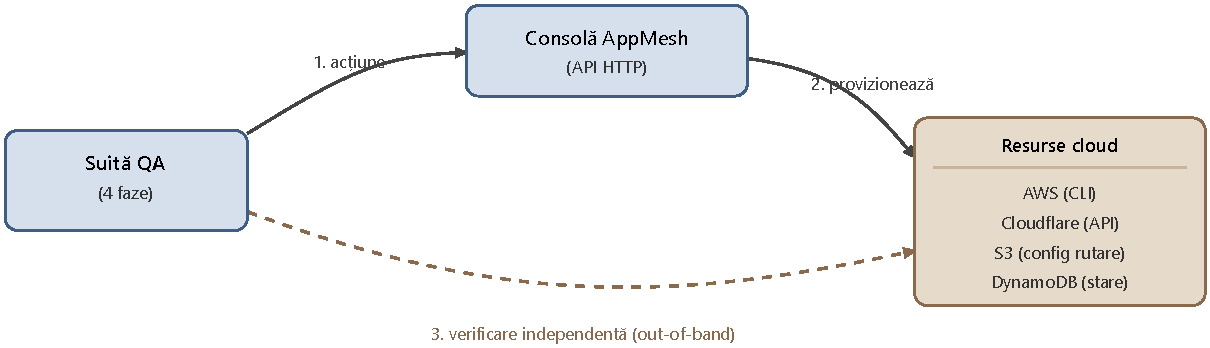
\includegraphics[width=0.82\textwidth]{pics/fig_oob.pdf}
\caption{Verificarea out-of-band: suita confirmă efectul fiecărei acțiuni citind direct din resursele cloud, independent de raportul consolei}
\label{fig:oob}
\end{figure}

Concret, suita interoghează AWS prin linia de comandă pentru a confirma existența și starea grupului de securitate, a launch template-ului, a Auto Scaling Group-ului, a target group-ului și a regulii de listener de pe ALB. Prin API-ul Cloudflare verifică înregistrările DNS, origin pool-urile și componența load balancer-ului global. Citește și parsează fișierul de configurație de rutare din S3, comparând ETag-ul înainte și după fiecare modificare pentru a confirma că o nouă configurație a fost într-adevăr publicată. Starea deployment-urilor și a conturilor este citită direct din tabelele DynamoDB. Fragmentul de cod din Figura~\ref{lst:oob} ilustrează o astfel de verificare, în care prezența serviciului și a regiunilor sale este confirmată citind configurația publicată în S3.

\begin{lstlisting}[language=Python]
# Verificare independenta: serviciul si regiunile lui trebuie sa apara
# in configuratia de rutare publicata in S3 (nu in raportul consolei).
cfg, etag = dump_gateway_config()
svcs = ((cfg or {}).get("gateway") or {}).get("services", {})
if SVC_NAME in svcs:
    regions = [r["name"] for r in svcs[SVC_NAME].get("regions", [])]
    if REGION in regions:
        ok(f"S3 gateway config: '{SVC_NAME}' contine regiunea '{REGION}'")
    else:
        fail(f"Regiunea '{REGION}' lipseste: {regions}")
else:
    fail(f"Serviciul '{SVC_NAME}' absent din config (ETag={etag})")
\end{lstlisting}
\captionof{figure}{Verificare out-of-band a configurației de rutare, citită direct din S3}\label{lst:oob}

\section{Trasabilitatea cerințelor}
Pentru a confirma că testarea are o acoperire completă, fiecare cerință funcțională din capitolul al doilea a fost pusă în corespondență cu fazele și scenariile ce o validează (Figura~\ref{fig:trasab}). Cerințele nefuncționale sunt acoperite indirect: securitatea accesului de către faza 1, disponibilitatea și reziliența de către fazele 3 și 4, iar observabilitatea prin apelarea endpoint-urilor de health-check pe tot parcursul.

\begin{figure}[t]
\centering
\small\linespread{1.05}\selectfont
\begin{tabular}{@{}p{1.7cm}p{12.6cm}@{}}
\toprule
\textbf{Cerință} & \textbf{Validată prin} \\
\midrule
CF1 & Faza 2-A: provizionarea unei aplicații dintr-o singură acțiune, cu verificarea fiecărei resurse din lanț (security group, rol, launch template, ASG, target group, regulă de listener, DNS). \\
CF2 & Faza 2: urmărirea stării pas cu pas până la \texttt{deployed}; faza 1: endpoint-urile de stare ale consolei. \\
CF3 & Faza 4-A, 4-B și 4-E: adăugarea unei regiuni, rularea aceluiași serviciu în două regiuni și gestionarea lor individuală. \\
CF4 & Faza 4-C: rutarea pe baza path-ului prin gateway către serviciul corect. \\
CF5 & Faza 4-D: failover indus prin defectarea regiunii primare și evitarea ei până la revenire. \\
CF6 & Faza 4-A: includerea origin pool-ului regiunii în load balancer-ul global Cloudflare. \\
CF7 & Faza 2-A și 4-D: starea target group-ului și deschiderea circuit breaker-ului pe baza health-check-urilor. \\
CF8 & Faza 2 și 4: modificarea ETag-ului configurației din S3 și concordanța cu starea din DynamoDB la fiecare schimbare. \\
CF9 & Faza 2-D, faza 3 și faza 4-E: deprovizionarea controlată, cu eliberarea tuturor resurselor asociate. \\
CF10 & Faza 1-A, 1-B, 1-C și 1-D: autentificarea, restricționarea operațiilor de administrator și izolarea între operatori. \\
\bottomrule
\end{tabular}
\caption{Matricea de trasabilitate a cerințelor funcționale către fazele și scenariile de testare}
\label{fig:trasab}
\end{figure}

\section{Rezultate}
La finalul campaniei de testare, toate verificările trec, după remedierea defectelor descrise în secțiunea următoare. Tabelul din Figura~\ref{fig:rezultate} rezumă acoperirea și rezultatul fiecărei faze. Fazele 2 și 3 au trecut fără defecte de la prima rulare completă; majoritatea problemelor au apărut, așa cum era de așteptat, în faza 4, partea cea mai complexă, care implică realizarea operațiilor pe trei sisteme distincte (AWS, Cloudflare și gateway-ul custom).

\begin{figure}[H]
\centering
\begin{tabular}{@{}p{1.6cm}p{8.6cm}p{2.4cm}@{}}
\toprule
\textbf{Faza} & \textbf{Acoperire} & \textbf{Rezultat} \\
\midrule
Faza 1 & Autentificare, autorizare, conturi, izolare între operatori, validarea formularului de deploy, tratarea erorilor, scanarea infrastructurii. & Trecută; 3 defecte remediate \\
Faza 2 & Provizionare cu verificare completă, scalare 1--3--1, actualizare artefact, deprovizionare. & Trecută; fără defecte \\
Faza 3 & Deprovizionare peste deconectare, deprovizionare întreruptă reluată, provizionare întreruptă cu rollback. & Trecută; fără defecte \\
Faza 4 & Adăugare regiune, rulare în două regiuni, rutare pe path, failover indus, eliminare regiune, revenire la starea de bază. & Trecută; 11 defecte remediate \\
\bottomrule
\end{tabular}
\caption{Rezultatele pe faze ale suitei de testare}
\label{fig:rezultate}
\end{figure}

\section{Defecte identificate și remediate}
Procesul de testare a scos la iveală paisprezece defecte. Treisprezece au fost corectate în cod, iar unul a constat într-o reglare a parametrilor de test (un timeout prea strâns pentru durata reală a unei deschideri de circuit breaker). Dincolo de cazurile individuale, defectele se grupează în câteva clase recurente, instructive pentru natura problemei.

Prima clasă ține de \textbf{eventual consistency} a serviciilor cloud: o resursă tocmai creată nu este imediat vizibilă, ceea ce poate produce verificări prematur eșuate sau pași care par să rateze deși vor reuși la scurt timp. A doua clasă ține de \textbf{idempotența deprovizionării}: o resursă deja inexistentă, ștearsă extern sau de o încercare anterioară, trebuie tratată ca un pas încheiat cu succes, nu ca o eroare, altfel un deployment rămâne blocat într-o stare parțială. A treia clasă privește \textbf{ordinea și cota operațiilor pe Cloudflare}: un origin pool nu poate fi șters cât timp este încă atașat load balancer-ului global, iar pool-urile orfane rămase după o deprovizionare incompletă consumă cota limitată de endpoint-uri (origini) a planului~\cite{cloudflare-pools}. O a patra clasă ține de \textbf{consecvența stării și a configurației}: după eliminarea unei regiuni, configurația de rutare din S3 trebuie resincronizată, iar fiecare regiune trebuie să citească propriul fișier de configurație.

\section{Scenariul de failover indus}
Cel mai relevant scenariu de validare este cel al failover-ului indus, care confirmă end-to-end cerințele privind rezistența la defectarea unei regiuni (CF5) și folosirea health-check-urilor în deciziile de rutare (CF7). Mecanismul intern pe care îl exercită este cel descris în capitolul al patrulea, ilustrat în Figura~\ref{fig:seq} și Figura~\ref{fig:cb}.

Scenariul pornește de la un serviciu pus în funcțiune în două regiuni, \texttt{us-east-1} și \texttt{eu-central-1}, și induce o defecțiune scalând la zero instanțe regiunea primară. În urma acestei acțiuni, target group-ul regional își marchează țintele ca unhealthy, iar monitorul gateway-ului, care interoghează health-check-ul la fiecare cincisprezece secunde, înregistrează eșecuri succesive. După trei eșecuri consecutive, circuit breaker-ul asociat perechii serviciu-regiune trece în starea \emph{Open}, iar gateway-ul începe să servească cererile din \texttt{eu-central-1}. Suita confirmă acest comportament repetând cereri către gateway și citind, din răspunsul serviciului demonstrativ, regiunea care a deservit cererea; failover-ul este considerat reușit atunci când răspunsul provine din regiunea secundară.

În a doua parte, scenariul restabilește regiunea primară, scalând-o înapoi la o instanță. După ce Auto Scaling Group-ul raportează din nou o instanță în serviciu și după întârzierea de treizeci de secunde a circuit breaker-ului, prima cerere readuce starea în \emph{Half-Open}, iar două probe reușite o readuc în \emph{Closed}, traficul revenind în regiunea primară. Acest ciclu complet, defectare urmată de revenire automată, fără intervenția operatorului și fără erori vizibile pentru utilizator, este transformat într-un comportament observabil de către aplicațiile demonstrative, care expun în fiecare răspuns regiunea și instanța ce au deservit cererea.

% ====================================================================
%  CAPITOLUL 7. EVALUARE EXPERIMENTALA
% ====================================================================
\chapter{Evaluare experimentală}

Dincolo de corectitudinea funcțională confirmată prin testare, acest capitol evaluează cantitativ comportamentul load balancer-ului propriu, partea centrală a platformei. Măsurătorile vizează patru aspecte: overhead-ul de latență introdus de gateway, comportamentul la failover-ul indus, viteza de revenire după repararea unei regiuni și latența cu care o schimbare de configurație se propagă în gateway. Toate valorile prezentate sunt măsurate pe platformă, nu estimate.

\section{Metodologia evaluării}
Evaluarea folosește load balancer-ul real, alături de două instanțe ale unui serviciu demonstrativ, rulate pe aceeași mașină pentru a izola comportamentul gateway-ului de variațiile rețelei. Cele două instanțe joacă rolul a două regiuni, \emph{local-a} și \emph{local-b}, iar gateway-ul își preia configurația de rutare din S3, prin exact același mecanism de route-sync folosit în producție. Parametrii sunt cei descriși în capitolul al cincilea: prag de trei eșecuri pentru deschiderea circuit breaker-ului, două probe reușite pentru închiderea lui, întârziere de treizeci de secunde înainte de o probă, health-check la fiecare cincisprezece secunde și un interval de poll de zece secunde pentru configurație.

Fiecare instanță își raportează propria identitate în pagina pe care o servește, astfel încât regiunea care deservește o cerere poate fi citită direct din răspuns. Pe baza acestei identități, măsurătorile disting fără ambiguitate regiunea primară de cea secundară. Întrucât instanțele rulează local, latențele absolute reflectă bucla locală, nu distanțe geografice reale; scopul măsurătorilor nu este latența de rețea, ci overhead-ul propriu al gateway-ului și dinamica mecanismelor de failover, recuperare și reîncărcare a configurației, care nu depind de distribuția geografică. Stratul global Cloudflare este distribuit geografic și ar folosi rețeaua de internet, astfel încât beneficiul de proximitate nu este cuantificat aici.

\section{Overhead-ul de rutare}
Pentru a măsura costul introdus de gateway, aceeași cerere a fost trimisă de două sute de ori direct către backend și de două sute de ori prin gateway, înregistrând latența fiecărei cereri. Toate cele patru sute de cereri au răspuns cu succes. Rezultatele sunt prezentate în Figura~\ref{fig:overhead}.

\begin{figure}[H]
\centering
\begin{tabular}{@{}p{4.2cm}rr@{}}
\toprule
\textbf{Latență (ms)} & \textbf{Direct} & \textbf{Prin gateway} \\
\midrule
Media        & 13,94 & 15,53 \\
Mediana      & 15,14 & 15,29 \\
P95          & 27,38 & 30,06 \\
P99          & 28,09 & 30,74 \\
Minim        & 2,39  & 4,23  \\
Maxim        & 28,38 & 31,78 \\
\bottomrule
\end{tabular}
\caption{Latența unei cereri, direct către backend și prin gateway (200 de cereri fiecare)}
\label{fig:overhead}
\end{figure}

Diferența dintre cele două coloane reprezintă overhead-ul propriu al gateway-ului, deoarece costul de procesare al backend-ului este aproape constant. Acesta este de aproximativ 1,59~ms în medie și 0,15~ms la mediană, cu o creștere de circa 2,7~ms la P95. Raportat la timpul total de deservire a unei cereri, overhead-ul introdus de selecția regiunii, gestionarea circuit breaker-ului și rescrierea path-ului este neglijabil.

\section{Failover indus}
Al doilea experiment reia scenariul de failover din capitolul anterior, de această dată măsurat. Cu serviciul activ în ambele regiuni și deservit din regiunea primară, instanța primară a fost oprită brusc, iar cererile au continuat să fie trimise prin gateway, la un ritm constant, timp de patruzeci de secunde. Din cele 146 de cereri trimise în timpul defecțiunii, niciuna nu a eșuat: prima cerere de după oprire a fost deja deservită din regiunea secundară, la numai 17~ms după producerea defecțiunii, prin retry-ul per-cerere al filtrului. La aproximativ cinci secunde, circuit breaker-ul regiunii primare a trecut în \emph{Open}, eliminând încercările ulterioare către regiunea oprită, în timp ce regiunea secundară a rămas \emph{Closed} și funcțională pe tot parcursul. Evoluția este redată în Figura~\ref{fig:fotimeline}.

\begin{figure}[H]
\centering
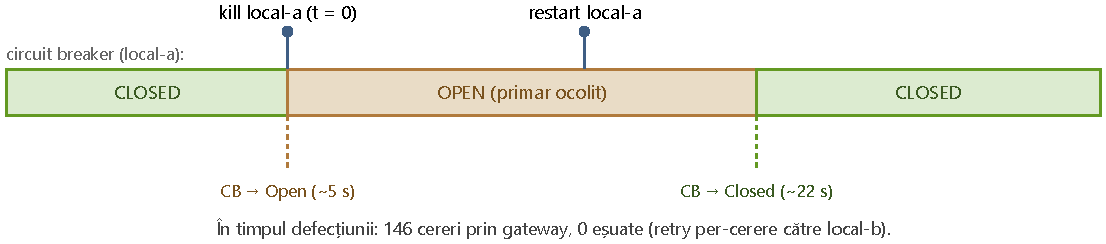
\includegraphics[width=0.95\textwidth]{pics/fig_failover_timeline.pdf}
\caption{Evoluția circuit breaker-ului regiunii primare la failover-ul indus și la recuperare}
\label{fig:fotimeline}
\end{figure}

Rezultatul confirmă proprietatea esențială a mecanismului: failover-ul se produce fără cereri eșuate și fără intervenția operatorului, iar circuit breaker-ul previne irosirea de timp pe o regiune defectă. Starea circuit breaker-elor expusă de gateway, în regim normal și în timpul defecțiunii, este prezentată în Figura~\ref{fig:sc-gwstatus}.

\section{Recuperarea după revenirea regiunii}
După fereastra de failover, instanța primară a fost repornită, iar cererile au continuat să fie monitorizate. Instanța a redevenit funcțională la 4,2~secunde după repornire, dar traficul nu a fost imediat redirecționat înapoi: circuit breaker-ul a rămas \emph{Open} până la expirarea întârzierii de probă, după care o probă a readus starea în \emph{Half-Open}, iar probele reușite l-au închis. Traficul a revenit în regiunea primară la aproximativ 22~secunde după repornire, moment confirmat la următoarea citire a stării circuit breaker-ului, devenită \emph{Closed}. Acest interval reflectă întârzierea de treizeci de secunde a circuit breaker-ului combinată cu ciclul de health-check, și reprezintă o revenire prudentă, menită să evite reintroducerea prematură a unei regiuni instabile.

\begin{lstlisting}
"ambulance-service": {                          // eu-central-1 functionala
  "mode": "multi-region-failover",
  "regions": [
    { "name": "eu-central-1", "circuitBreaker": "CLOSED", "healthy": true  },
    { "name": "us-east-1",    "circuitBreaker": "CLOSED", "healthy": true  } ]
}

"ambulance-service": {                          // eu-central-1 cazuta -> failover
  "mode": "multi-region-failover",
  "regions": [
    { "name": "eu-central-1", "circuitBreaker": "OPEN",   "healthy": false },
    { "name": "us-east-1",    "circuitBreaker": "CLOSED", "healthy": true  } ]
}
\end{lstlisting}
\captionof{figure}{Starea raportată de gateway la \texttt{/gateway/status} pentru \texttt{ambulance-service}: cu regiunea eu-central-1 funcțională (sus, ambele \emph{Closed}) și căzută (jos, eu-central-1 trecută în \emph{Open} și ocolită prin failover către us-east-1)}\label{fig:sc-gwstatus}

\section{Propagarea configurației}
Ultimul experiment măsoară cât de repede o schimbare de configurație ajunge în gateway, fără repornirea acestuia. Pornind de la un serviciu deservit din regiunea primară, configurația din S3 a fost modificată astfel încât serviciul să fie rutat exclusiv către cealaltă regiune. Gateway-ul a preluat noua configurație și a redirecționat traficul după 7,54~secunde, în limita unui singur ciclu de poll de zece secunde, fără nicio repornire și fără cereri eșuate. Acest rezultat confirmă că modificările de topologie luate în consolă se propagă către load balancere, în limita intervalului de poll.

\section{Sinteză și limitări}
Indicatorii măsurați sunt rezumați în Figura~\ref{fig:evalsumar}. Împreună, aceștia arată un gateway cu overhead propriu redus, un failover fără pierderi de cereri și o reîncărcare a configurației la cald, în limita intervalului de poll.

\begin{figure}[H]
\centering
\begin{tabular}{@{}p{8.8cm}p{4cm}@{}}
\toprule
\textbf{Indicator} & \textbf{Valoare măsurată} \\
\midrule
Overhead median introdus de gateway & 0,15 ms (media 1,59 ms) \\
Cereri eșuate în timpul failover-ului & 0 din 146 \\
Prima cerere deservită din regiunea secundară & la 17 ms după defectare \\
Deschiderea circuit breaker-ului & $\sim$5 s \\
Revenirea traficului la regiunea primară & $\sim$22 s după repornire \\
Propagarea unei schimbări de configurație & 7,54 s (poll de 10 s) \\
\bottomrule
\end{tabular}
\caption{Sinteza indicatorilor măsurați experimental}
\label{fig:evalsumar}
\end{figure}

Evaluarea are limitări asumate. Măsurătorile au fost realizate pe o singură mașină, cu două regiuni și un serviciu demonstrativ ușor, astfel încât latențele absolute reflectă bucla locală, iar beneficiul de latență al direcționării globale pe baza proximității, fiind o proprietate a geografiei, nu este cuantificat aici. Aceste limitări nu afectează însă concluziile privind overhead-ul propriu al gateway-ului, comportamentul la failover și recuperare, sau viteza de propagare a configurației, care țin de logica platformei și nu de distribuția geografică. O evaluare la scară geografică reală, pe mai multe regiuni, rămâne o direcție de continuare, discutată în capitolul de concluzii.

% ====================================================================
%  CAPITOLUL 8 — CONCLUZII ȘI DEZVOLTĂRI VIITOARE
% ====================================================================
\chapter{Concluzii și dezvoltări viitoare}

Acest capitol final recapitulează rezultatele obținute, raportându-le la obiectivele formulate în introducere, discută limitele soluției și conturează direcțiile în care platforma poate fi extinsă dincolo de stadiul atins în prezenta lucrare.

\section{Concluzii}
Lucrarea a pornit de la o problemă concretă a administrației publice: punerea în funcțiune și operarea aplicațiilor web guvernamentale presupune asamblarea coordonată a numeroase resurse de infrastructură, o sarcină repetitivă, dependentă de ordinea operațiilor și predispusă la erori atunci când este efectuată manual; efortul crește cu cât o instituție administrează un portofoliu întreg de aplicații, fiecare prezentă în mai multe regiuni. Răspunsul propus, AppMesh, este o platformă self-service care unifică sub o singură interfață întregul ciclu de viață al unei aplicații, de la provizionare până la administrarea traficului în exploatare, separând clar planul de control de planul de date.

Obiectivele specifice fixate în introducere au fost atinse și confirmate experimental. Punerea în funcțiune a unei aplicații este integral automatizată: pornind de la o singură acțiune în consolă, cei doisprezece pași de provizionare sunt executați în ordine, fără configurare manuală a vreunei resurse, iar deprovizionarea readuce sistemul la o stare curată în mod idempotent, fără a lăsa resurse orfane. Load balancer-ul multi-region custom rutează cererile pe baza path-ului și face failover automat către o regiune funcțională atunci când regiunea preferată devine indisponibilă, fără cereri eșuate și fără intervenția operatorului, după cum a arătat scenariul de failover indus. Direcționarea globală a utilizatorilor către cea mai apropiată regiune este asigurată de stratul Cloudflare, care reorientează automat traficul în caz de indisponibilitate. Sursa unică de adevăr privind configurația și starea aplicațiilor este menținută în planul de control și propagată la planul de date prin mecanismul de route-sync, astfel încât load balancerele reflectă în permanență deciziile luate în consolă. În sfârșit, întreaga soluție a fost validată pe o infrastructură reală, găzduind servicii guvernamentale demonstrative pentru ambulanță și poliție.

Dincolo de funcționalitate, evaluarea experimentală a cuantificat comportamentul componentei centrale, load balancer-ul propriu, arătând un overhead de rutare neglijabil, un failover fără pierderi de cereri, o revenire prudentă după repararea unei regiuni și o propagare a configurației în limita intervalului de poll. Procesul de testare, organizat în patru faze și dublat de o verificare out-of-band a efectelor asupra infrastructurii, a confirmat corectitudinea funcțională și a scos la iveală mai multe clase de defecte specifice operării în cloud, remediate ulterior. Per ansamblu, lucrarea demonstrează că o instituție poate administra un portofoliu de aplicații web disponibile și scalabile dintr-un singur punct de control, cu un efort operațional considerabil redus față de gestionarea manuală a fiecărei componente.

\section{Limitări}
Soluția prezentată are câteva limite, rezultate din deciziile luate pentru realizarea prototipului. Ele nu afectează validitatea concluziilor privind logica platformei, dar marchează granița dintre ceea ce a fost implementat și ceea ce ar necesita o implementare de producție.

Prima limitare ține de \textbf{partajarea load balancer-ului regional}. În implementarea curentă, consola, gateway-ul și aplicațiile din aceeași regiune sunt deservite de un singur ALB, prin reguli de listener pe bază de host, decizie motivată de costul fix lunar al fiecărui ALB, semnificativ în contextul unui prototip. Consecința este că stratificarea logică a sistemului nu este impusă și la nivel de rețea: aplicațiile rămân direct accesibile prin host-ul propriu, ocolind gateway-ul și, odată cu el, rutarea pe path, failover-ul și circuit breaker-ul, iar suprafața de administrare a consolei este expusă pe același ingress public ca traficul aplicațiilor.

A doua limitare ține de \textbf{stratul global de direcționare}. Abonamentul Cloudflare utilizat pentru realizarea prototipului permite un număr fix de endpoint-uri (origini) într-un origin pool, ceea ce restrânge la două numărul de regiuni între care se poate face failover la nivel global~\cite{cloudflare-pools}. Mecanismul intern al gateway-ului nu are această limită, însă direcționarea globală pe baza proximității, care reorientează utilizatorii între regiuni, este plafonată de cota abonamentului.

A treia limitare ține de \textbf{mediul de evaluare}. Măsurătorile cantitative au fost realizate pe o singură mașină, cu două regiuni simulate prin instanțe locale și un serviciu demonstrativ ușor. Această configurație izolează corect overhead-ul propriu al gateway-ului și dinamica mecanismelor de failover, recuperare și propagare a configurației, dar nu poate cuantifica beneficiul de latență al direcționării globale pe baza proximității, care este o proprietate a distribuției geografice reale și a rețelei.

\section{Dezvoltări viitoare}
Limitările de mai sus indică direct primele direcții de continuare. Separarea ingress-ului ar înlocui ALB-ul regional partajat cu o topologie stratificată, în care consola dispune de un ALB propriu, restricționat (de exemplu la nivel de CIDR sau intern instituției), gateway-ul de un ALB public dedicat, care rămâne singura poartă de intrare către aplicații, iar aplicațiile de un ALB intern comun, accesibil exclusiv prin gateway. O astfel de topologie ar impune și la nivel de rețea stratificarea pe care platforma o presupune la nivel logic, eliminând accesul direct la aplicații și scoțând suprafața de administrare de pe ingress-ul public. Extinderea dincolo de două regiuni la nivelul direcționării globale ar presupune fie un plan cu o cotă mai mare de endpoint-uri, fie un mecanism alternativ de steering global, astfel încât failover-ul la nivel de regiune să poată cuprinde un număr arbitrar de regiuni. Nu în ultimul rând, o evaluare la scară geografică reală, cu gateway-uri deployate în regiuni AWS distincte, ar permite măsurarea câștigului de latență adus de proximitate și validarea failover-ului la distanțe de rețea reale, completând rezultatele obținute local.

Dincolo de acestea, platforma se pretează la mai multe extinderi care i-ar consolida utilitatea operațională:

\begin{itemize}
	\item \textbf{Observabilitate centralizată}, prin agregarea metricilor și a jurnalelor de la gateway-uri și de la aplicații într-un tablou de bord unic, care să ofere operatorului o imagine în timp real asupra stării regiunilor, a traficului și a declanșărilor de failover.
	\item \textbf{Strategii avansate de deployment}, precum actualizările de tip blue-green sau canary, care ar permite înlocuirea versiunii unei aplicații fără întreruperea serviciului, integrate în lanțul de provizionare existent.
	\item \textbf{Întărirea securității}, prin adăugarea unui web application firewall pe ingress-ul public, autentificare reciprocă (mTLS) între gateway și aplicațiile interne și o gestiune dedicată a secretelor, în special în contextul serviciilor guvernamentale.
	\item \textbf{Politici de scalare mai fine}, bazate pe metrici specifice aplicației, nu doar pe gradul de utilizare a procesorului, pentru a adapta mai precis numărul de instanțe la natura sarcinii.
\end{itemize}

Aceste direcții pornesc de la o platformă deja funcțională și validată, confirmând că abordarea aleasă, centrarea pe o sursă unică de adevăr și separarea planului de control de planul de date, oferă o bază solidă pe care administrarea aplicațiilor web guvernamentale poate fi dusă mai departe.

\bibliographystyle{plain}
\bibliography{bibliography}

\end{document}
